\newcommand{\precDTL}{5} % TODO choose something larger than k for smallest 1e-k
                         %      ever seen in plots
In diesem abschließenden Kapitel möchten wir nun die in
\Cref{chap:implementation} beschriebene Realisierung von
\Cref{alg:primalDualIteration} mit Abbruchkriterium
\eqref{eq:terminationCriterion} im Solve-Schritt der AFEM-Schleife aus
\Cref{fig:afemLoop} an einigen Benchmark-Problemen untersuchen.
Dabei benutzen wir die Bezeichnungen aus \Cref{alg:primalDualIteration} und
schreiben $\ucrt$ für $\ucr$ sowie $\bar\Lambda_{0,\Tcal}$ für $\bar\Lambda_0$
aus \Cref{thm:convergenceIteration} bezüglich einer Triangulierung $\Tcal$ .
Zunächst möchten wir alle Parameterwahlen aufführen, die in allen 
Experimenten gleich gesetzt werden, sofern nicht anders angegeben.
Als Startwert für die Iteration auf dem ersten Level wählen wir
$u_0\equiv 0$ und auf den darauffolgenden Leveln eine Prolongation wie zum
Ende von \Cref{sec:programFlow} beschrieben, womit die Wahl des Startwerts
der ersten Levels keinen nennenswerten Einfluss auf die Dauer des Experiments
oder die Güte der Ergebnisse hat. 
Für jeden Aufruf der primalen-dualen Iteration wählen wir $\Lambda_0$ wie in
\Cref{eq:choiceInitialDualVariableImplementation} angegeben.
Dabei konstruieren wir Probleme, bei denen die exakte Lösung bekannt ist,
nach \Cref{sec:constructionInputSignal}. 
Bei diesen ist ein Argument $r$ stets aus $[0,\infty)$.
\begin{table}[p]
  \centering
  \begin{tabular}{c|c}
    \hline 
    Parametername & Standardwert\\
    \hline 
    \texttt{degree4Integrate}&
    $10$\\
    \texttt{geometry} &
    \texttt{'BigSquare'} (\texttt{'Square'})\\
    \texttt{parTheta} &
    $0.5$\\
    \texttt{minNrDof} &
    $10^8$\\
    \texttt{useProlongation} &
    \texttt{true}\\
    \texttt{parGamma} &
    $1$\\
    \texttt{u0Mode} &
    \texttt{zeros}\\
    \texttt{epsStop} &
    $10^{-4}$\\
    \texttt{parTau} &
    $1$\\
    \texttt{maxIter} &
    $10^{12}$\\
    \texttt{parAlpha} &
    $1$ ($10^4$)\\
    \hline
  \end{tabular}
  \caption{Parameter für Experiment mit Funktion als Eingangssignal, für welche
  die exakte Lösung bekannt ist und in Klammern die Werte für ein 
  Graufarbenbild als Eingangssignal, falls sich diese unterscheiden}
  \label{tab:parameterStandardValues}
\end{table} 
Eine Übersicht über die Wahl aller für die Experimente relevanten Parameter aus
den Tabellen \ref{tab:paramsMisc}--\ref{tab:paramsExperiment}, deren Wahl in
diesem und den folgenden beiden Abschnitten \ref{sec:choiceOfParameters} und
\ref{sec:experimentsWithExactSolution}, teilweise auch experimentell, begründet
wird, ist in der Tabellen \ref{tab:parameterStandardValues} zu finden.
Diese werden immer so gewählt, wenn nicht explizit etwas anderes angegeben
wird.
Als besonderes Augenemerk betrachten wir dabei zunächst zwei Eingangssignale,
um in einigen Experimenten in \Cref{sec:choiceOfParameters} die Parameter für
die primale-duale Iteration zu ermitteln, die in allen weiteren Experimenten
genutzt werden sollen.
Andere Funktionen werden wir bei Bedarf betrachten, um bestimmte Eigenschaften
zu untersuchen im Vergleich zu diesen beiden Benchmark-Problemen.
Für ein Experiment mit exakter Lösung betrachten wir für einen Parameter
$\beta\geq 1/2$, wobei wir $\beta =1$ wählen, die Funktion
\begin{align*}
  u(r)&\coloneqq
  \begin{cases}
    1, 
    & \text{falls } r\in \left[0,\frac{1}{6}\right]\!,\\
    1+(6r-1)^\beta, 
    & \text{falls } r\in \left(\frac{1}{6}, \frac{1}{3}\right]\!,\\
    2, 
    & \text{falls } r\in \left(\frac{1}{3}, \frac{1}{2}\right]\!,\\
    2\left(\frac{5}{2}-3r\right)^\beta, 
    & \text{falls } r\in \left(\frac{1}{2}, \frac{5}{6}\right]\!,\\
    0, 
    & \text{falls } r\in \left(\frac{5}{6}, \infty\right)\!,\\
  \end{cases}
\end{align*}
und wählen
\begin{align*}
  \sgn\big(\partial_r u(r)\big) 
  &\coloneqq
  \begin{cases}
    12r-36r^2, 
    & \text{falls } r\in \left[0,\frac{1}{6}\right]\!,\\
    1, 
    & \text{falls } r\in \left(\frac{1}{6}, \frac{1}{3}\right]\!,\\
    \cos(\pi(6r-2)), 
    & \text{falls } r\in \left(\frac{1}{3}, \frac{1}{2}\right]\!,\\
    -1, 
    & \text{falls } r\in \left(\frac{1}{2}, \frac{5}{6}\right]\!,\\
    -\frac{1+\cos(\pi(6r-5))}{2}, 
    & \text{falls } r\in \left(\frac{5}{6}, \infty\right)\!.
  \end{cases}
\end{align*}
Nach \Cref{eq:constructionInputSignal} ist $u$ mit dieser Wahl von
$\sgn\big(\partial_r u\big)$ die Lösung von \Cref{prob:continuousProblem} mit
Eingangssignal
\begin{align}
  \label{eq:inputSignalF01}
  f_\alpha(r)
  &=
  \begin{cases}
    \alpha-12(2-9r), 
    & \text{falls } r\in \left[0,\frac{1}{6}\right]\!,\\
    \alpha\left(1+(6r-1)^\beta\right)-\frac{1}{r}, 
    & \text{falls } r\in \left(\frac{1}{6}, \frac{1}{3}\right]\!,\\
    2\alpha+6\pi\sin(\pi(6r-2))-\frac{1}{r}\cos(\pi(6r-2)), 
    & \text{falls } r\in \left(\frac{1}{3}, \frac{1}{2}\right]\!,\\
    2\alpha\left(\frac{5}{2}-3r\right)^\beta+\frac{1}{r},
    & \text{falls } r\in \left(\frac{1}{2}, \frac{5}{6}\right]\!,\\
    -3\pi\sin(\pi(6r-5))+\frac{1+\cos(\pi(6r-5))}{2r}, 
    & \text{falls } r\in \left(\frac{5}{6}, \infty\right)\!.
  \end{cases}
\end{align}
Das Eingangssignal $f_\alpha$ für zwei Wahlen von $\alpha$ und die exakte
Lösung $u$ können in \Cref{fig:f01Plots} betrachtet werden.
Wir können anhand von \Cref{fig:f01Plots} auch feststellen, dass für große
$\alpha$ die Interpretation des ROF-Modells aus \Cref{chap:introduction}
zutrifft, denn rein optisch gilt für $\alpha=10^4$ annähernd $f_\alpha=\alpha
u$.
Ebenfalls nach \Cref{sec:constructionInputSignal} können die schwachen
Gradienten von $u$ und $f_\alpha$ bestimmt werden mithilfe der partiellen 
Ableitungen
\begin{align*}
  \partial_r f_\alpha(r)
  &=
  \begin{cases}
    108,
    & \text{falls } r\in\left[0,\frac{1}{6}\right]\!,\\
    6\alpha\beta(6r-1)^{\beta-1} +\frac{1}{r^2}, 
    & \text{falls } r\in\left(\frac{1}{6},\frac{1}{3}\right]\!,\\
    \left(36\pi^2+\frac{1}{r^2}\right)\cos(\pi(6r-2))
    + \frac{6\pi}{r}\sin(\pi(6r-2)), 
    & \text{falls } r\in\left(\frac{1}{3},\frac{1}{2}\right]\!,\\
    -\left(6\alpha\beta\left( \frac{5}{2}-3r \right)^{\beta-1}+
    \frac{1}{r^2}\right),
    & \text{falls } r\in\left(\frac{1}{2},\frac{5}{6}\right]\!,\\
    -\left( \left( 18\pi^2+\frac{1}{2r^2} \right)\cos(\pi(6r-5))
    +\frac{1}{2r^2} + \frac{3\pi}{r}\sin(\pi(6r-5))\right)\!, 
    &\text{falls } r\in\left(\frac{5}{6},\infty\right)\!,
  \end{cases}
\end{align*}
und 
\begin{align*}
  \partial_r u(r) 
  &= 
  \begin{cases}
    0,
    & \text{falls } r\in\left[0,\frac{1}{6}\right]\!,\\
    6\beta(6r-1)^{\beta-1}, 
    & \text{falls } r\in\left(\frac{1}{6},\frac{1}{3}\right]\!,\\
    0, 
    & \text{falls } r\in\left(\frac{1}{3},\frac{1}{2}\right]\!,\\
    -6\beta\left( \frac{5}{2}-3r \right)^{\beta-1},
    & \text{falls } r\in\left(\frac{1}{2},\frac{5}{6}\right]\!,\\
    0,
    &\text{falls } r\in\left(\frac{5}{6},\infty\right)\!.
  \end{cases}
\end{align*} 
Durch Kenntnis des schwachen Gradienten von $u$ erhalten wir
für die exakte Energie die Approximation
$
\DTLloaddb{db}{data/paramsReducedStandardF01.csv}
\DTLassign{db}{1}{\exactEnergy=exactEnergy} 
\DTLgdeletedb{db}
E(u)\approx\DTLround{\exactEnergy}{\exactEnergy}{\precDTL}\exactEnergy
$ für das Experiment mit $\alpha=1$ und
$
\DTLloaddb{db}{data/paramsReducedStandardF01Alpha1e4.csv}
\DTLassign{db}{1}{\exactEnergy=exactEnergy} 
\DTLgdeletedb{db}
E(u)\approx\DTLround{\exactEnergy}{\exactEnergy}{\precDTL}\exactEnergy
$ für das Experiment mit $\alpha=10^4$,
mit denen wir die jeweiligen Ergebnisse der Experimente vergleichen können.
\begin{figure}[p]
  \centering
  \begin{subfigure}[b]{.48\linewidth}
    \centering
    \caption{$f_1$}
    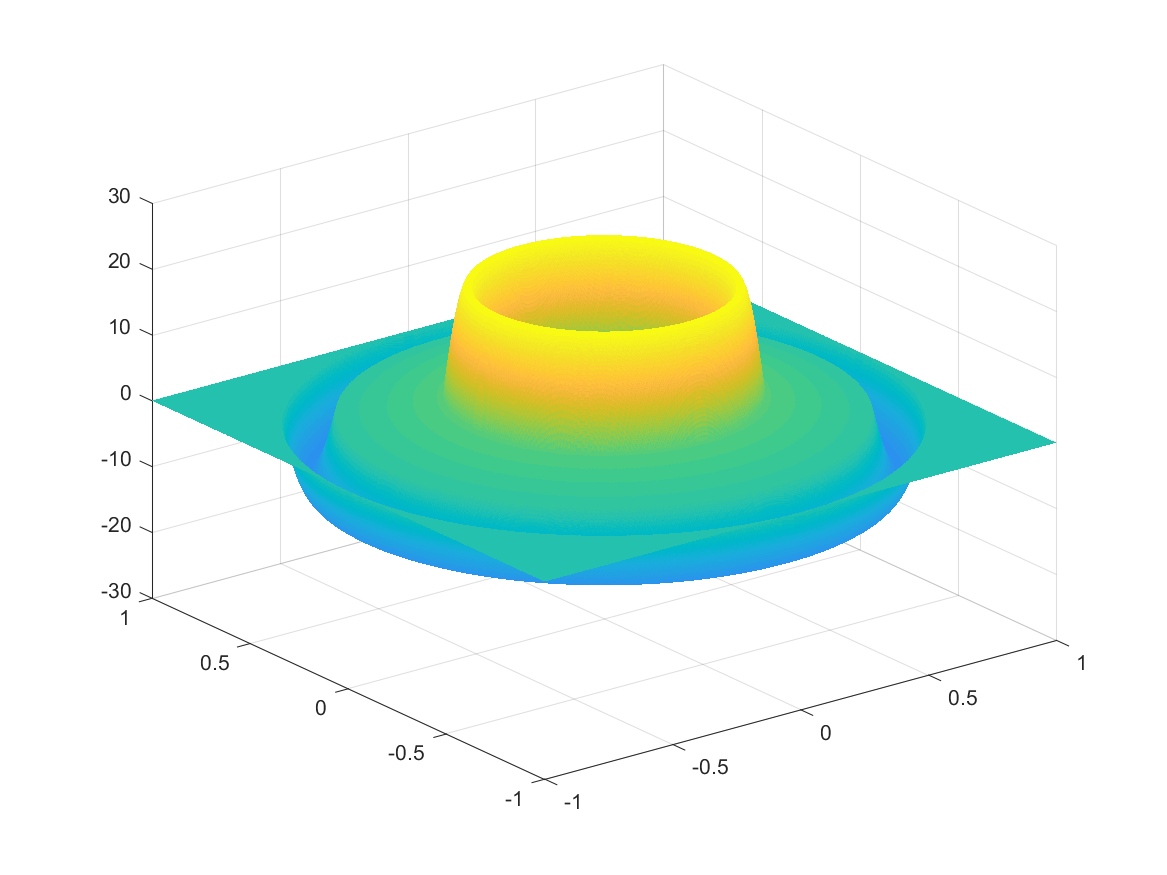
\includegraphics[trim = 40 30 30 30, clip, width=\linewidth]
      {pictures/chapExperiments/secGeneralInfo/f01Plots/inSi1.png}
    \label{fig:f01InSi}
  \end{subfigure}
  \quad
  \begin{subfigure}[b]{.48\linewidth}
    \centering
    \caption{$f_1$ entlang der x- und y-Achse}
    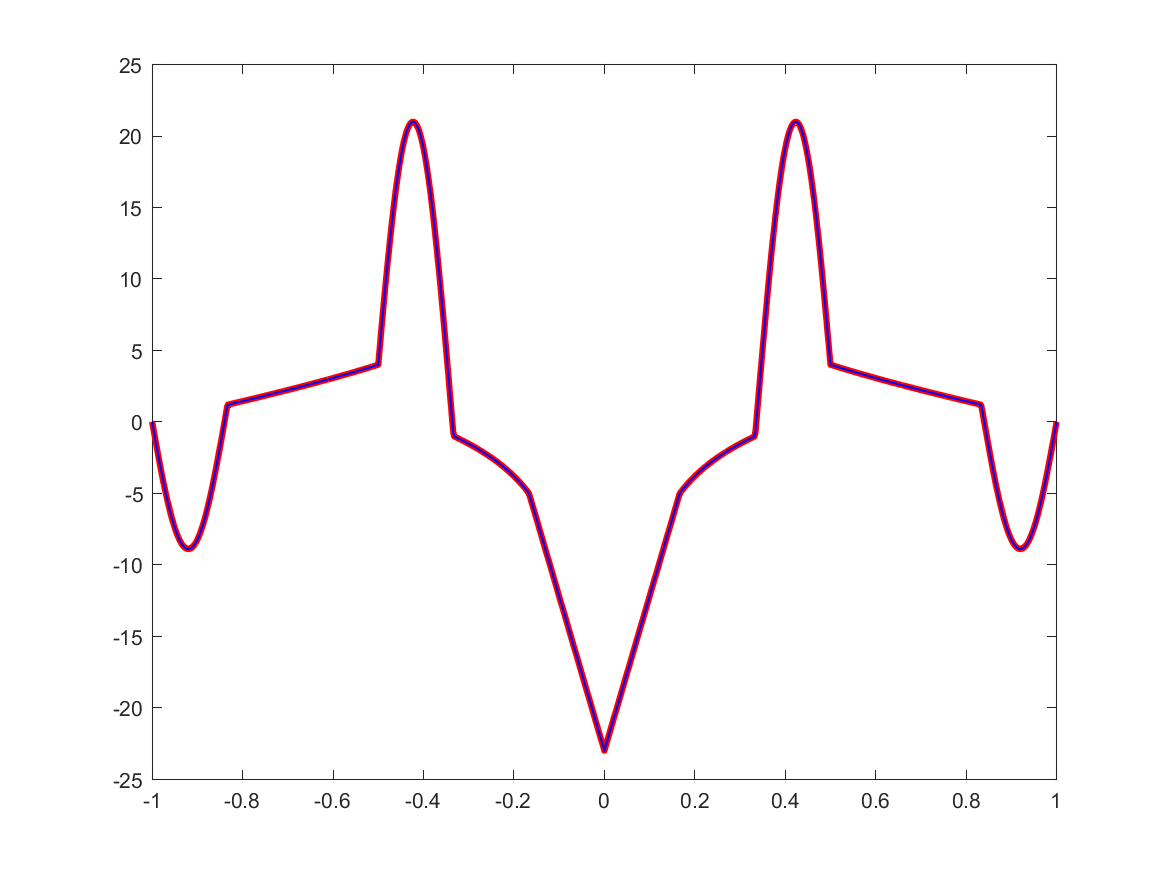
\includegraphics[trim = 50 30 50 20, clip, width=\linewidth]
      {pictures/chapExperiments/secGeneralInfo/f01Plots/inSi1Axis.png}
    \label{fig:f01InSiAxis}
  \end{subfigure}

  \begin{subfigure}[b]{.48\linewidth}
    \centering
    \caption{$f_{10^4}$}
    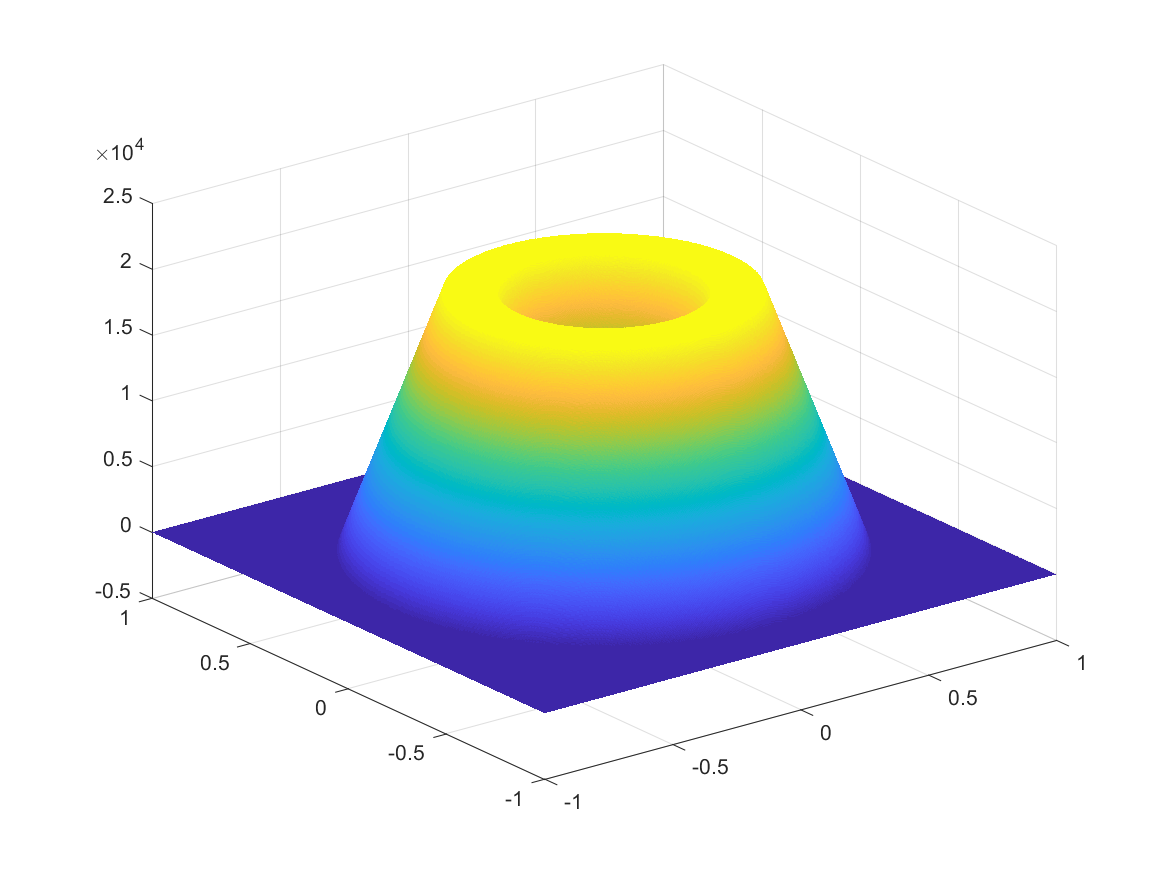
\includegraphics[trim = 40 30 30 30, clip, width=\linewidth]
      {pictures/chapExperiments/secGeneralInfo/f01Plots/inSi1e4.png}
    \label{fig:f01AlphaLargeInSi}
  \end{subfigure}
  \quad
  \begin{subfigure}[b]{.48\linewidth}
    \centering
    \caption{$f_{10^4}$ entlang der x- und y-Achse}
    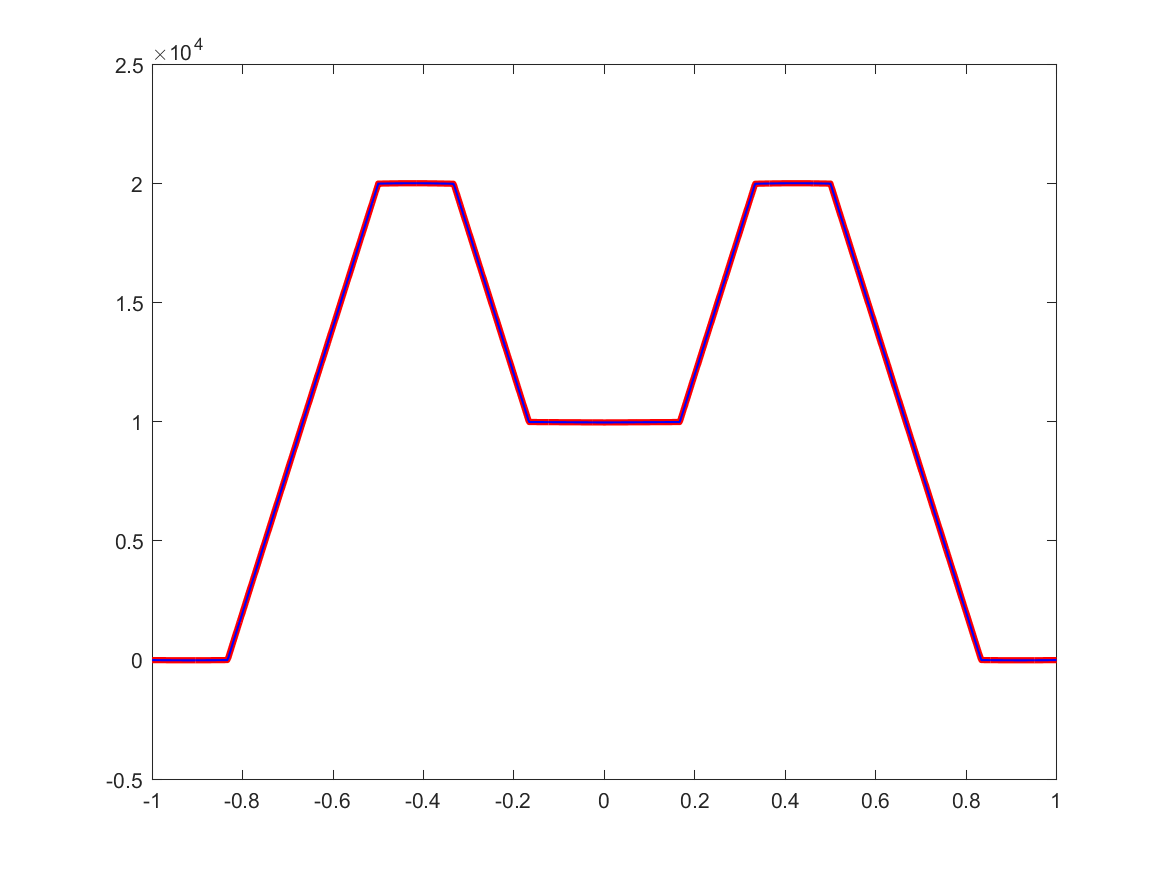
\includegraphics[trim = 50 30 50 20, clip, width=\linewidth]
      {pictures/chapExperiments/secGeneralInfo/f01Plots/inSi1e4Axis.png}
    \label{fig:f01AlphaLargeInSiAxis}
  \end{subfigure}

  \begin{subfigure}[b]{.48\linewidth}
    \centering
    \caption{$u$}
    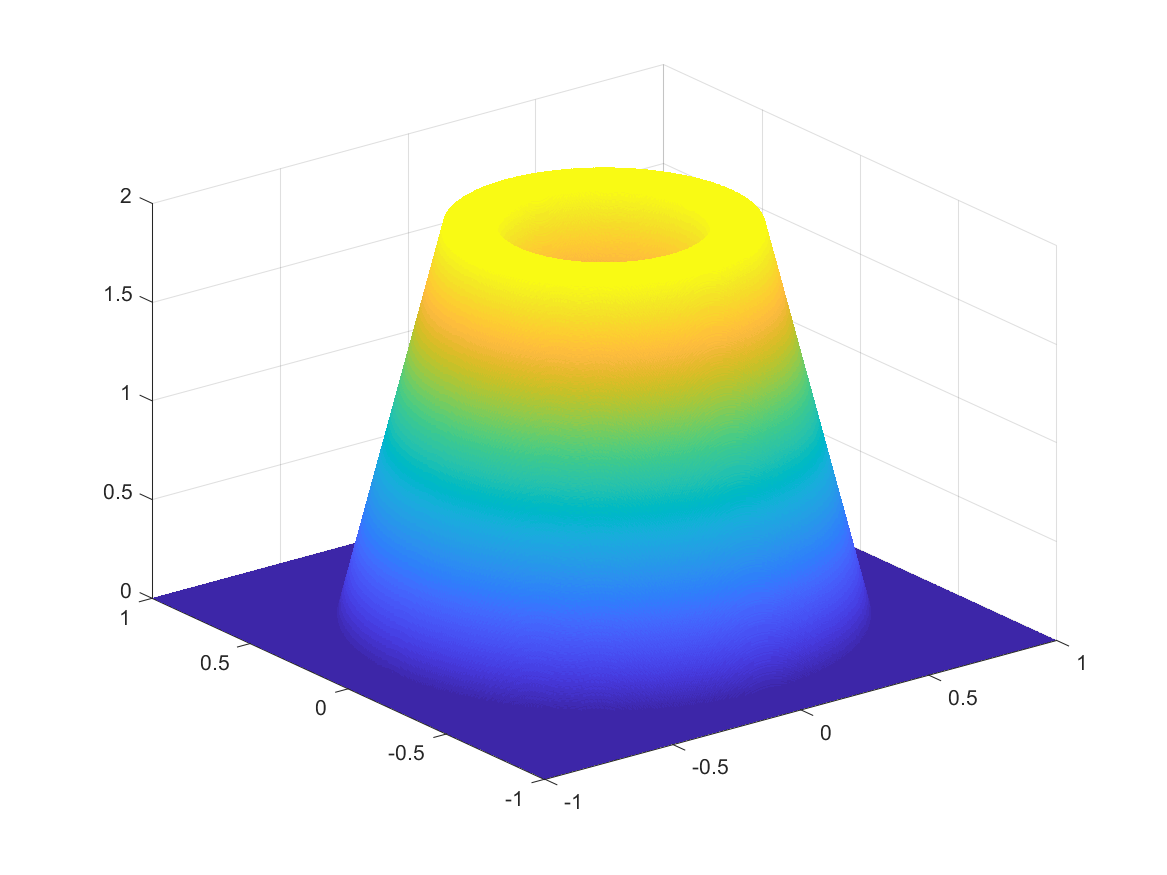
\includegraphics[trim = 40 30 30 30, clip, width=\linewidth]
      {pictures/chapExperiments/secGeneralInfo/f01Plots/exactSolution.png}
    \label{fig:f01ExactSol}
  \end{subfigure}
  \quad
  \begin{subfigure}[b]{.48\linewidth}
    \centering
    \caption{$u$ entlang der x- und y-Achse}
    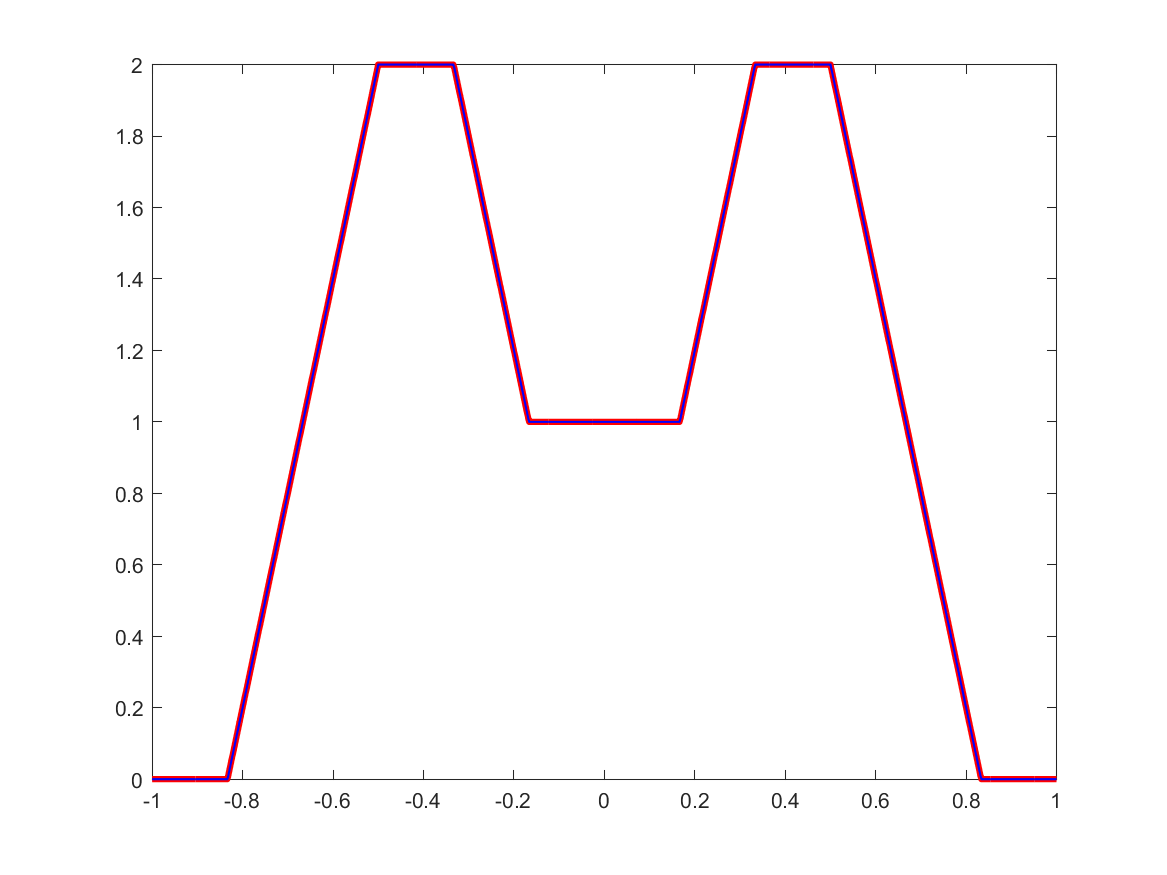
\includegraphics[trim = 50 30 50 20, clip, width=\linewidth]
      {pictures/chapExperiments/secGeneralInfo/f01Plots/exactSolutionAxis.png}
    \label{fig:f01ExactSolAxis}
  \end{subfigure} 
  \caption{Eingangssignal $f_\alpha$ und exakte Lösung $u$ sowie deren
  Darstellungen entlang der x-Achse (blau) und der y-Achse (rot) für
  $\alpha\in\{1,10^4\}$.}
  \label{fig:f01Plots}
\end{figure}
Als initiale Geometrie, das heißt die Geometrie für das erste Level des
AFEM-Al\-go\-rith\-mus, nutzen wir in den Experimenten mit exakter Lösung
\texttt{BigSquare} des AFEM-Pakets ohne initiale Rotverfeinerung, zu sehen in
\Cref{fig:triangBigSquare}, da diese den Einheitskreis, das heißt den Träger
des Eingangssignals und der exakten Lösung nach
\Cref{sec:constructionInputSignal}, enthält.
Wenn nicht anders angegeben, dann betrachten wir dieses Beispiel stets mit
$\alpha=1$, also mit Eingangssignal $f_1$. 
Diese Wahl für $\alpha$ tätigen wir auch für die anderen Probleme mit 
exakter Lösung, falls nichts anderes angegeben ist.

Für ein Problem mit unstetigem Eingangssignal legen wir besonderes
Augenmerk auf das Graufarbenbild \texttt{cameraman} aus \cref{fig:cameraman}
als Eingangssignal. 
Wir betrachten dieses Beispiel stets mit $\alpha=10^4$.
Auch für dieses komplexere Beispiel, bei der selbst eine stückweise
Beschreibung durch Polynome augenscheinlich nur schwer möglich ist, sowie in
allen weiteren Experimenten haben selbst deutlich höhere Integrationsgrade als
$10$ zu keinen veränderten Raten geführt. 
Diese Wahl des Integrationsgrads erscheint daher als ausreichend.
Da außerdem in dieser Implementierung darauf geachtet wurde, die
\texttt{integrate} Methode des AFEM-Softwarepakets \cite{Car09} nicht während
der primalen-dualen Iteration aufzurufen, hat eine möglicherweise zu hohe Wahl
des Integrationsgrads keinen relevanten Effekt auf die Programmlaufzeit und
kann somit ohne Sorge als 10 gewählt werden.
Diese Wahl des Integrationsgrads gilt nur für die Methode \texttt{errorCRL2}
des AFEM-Softwarepakets zur Berechnung des Fehlers nicht, da diese unverändert
übernommen wurde und den Grad 12 nutzt.
Fur Experiment mit Graufarbenbild als Eingangssignal nutzen wir als initiale
Triangulierung \texttt{Square} des AFEM-Softwarepakets ohne initiale
Rotverfeinerung, zu sehen in \Cref{fig:triangSquare}.

\begin{figure}[p]
  \centering
  \begin{subfigure}[b]{.48\linewidth}
    \centering
    \caption{\texttt{BigSquare}}
    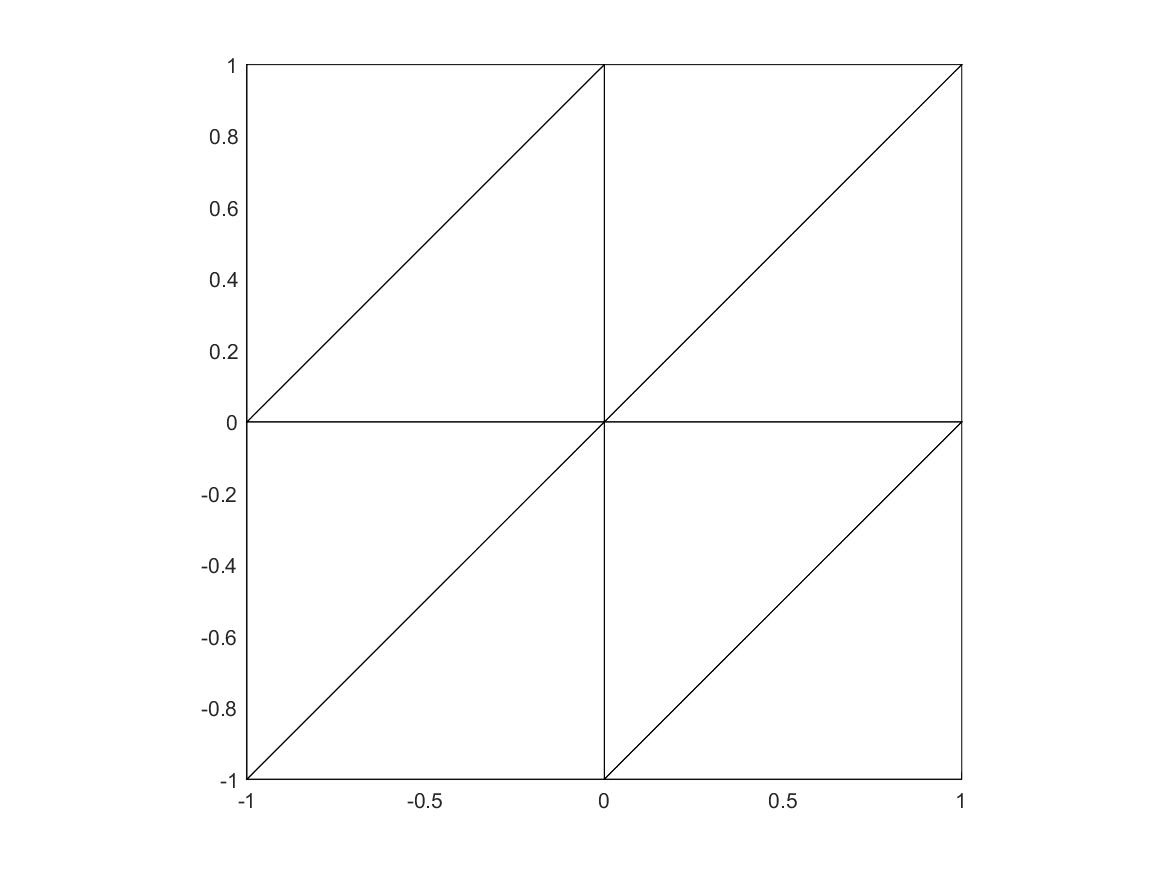
\includegraphics[trim = 90 30 90 20, clip, width=\linewidth]
      {pictures/chapExperiments/secGeneralInfo/bigSquareTriang.png}
    \label{fig:triangBigSquare}
  \end{subfigure}
  \quad
  \begin{subfigure}[b]{.48\linewidth}
    \centering
    \caption{\texttt{Square}}
    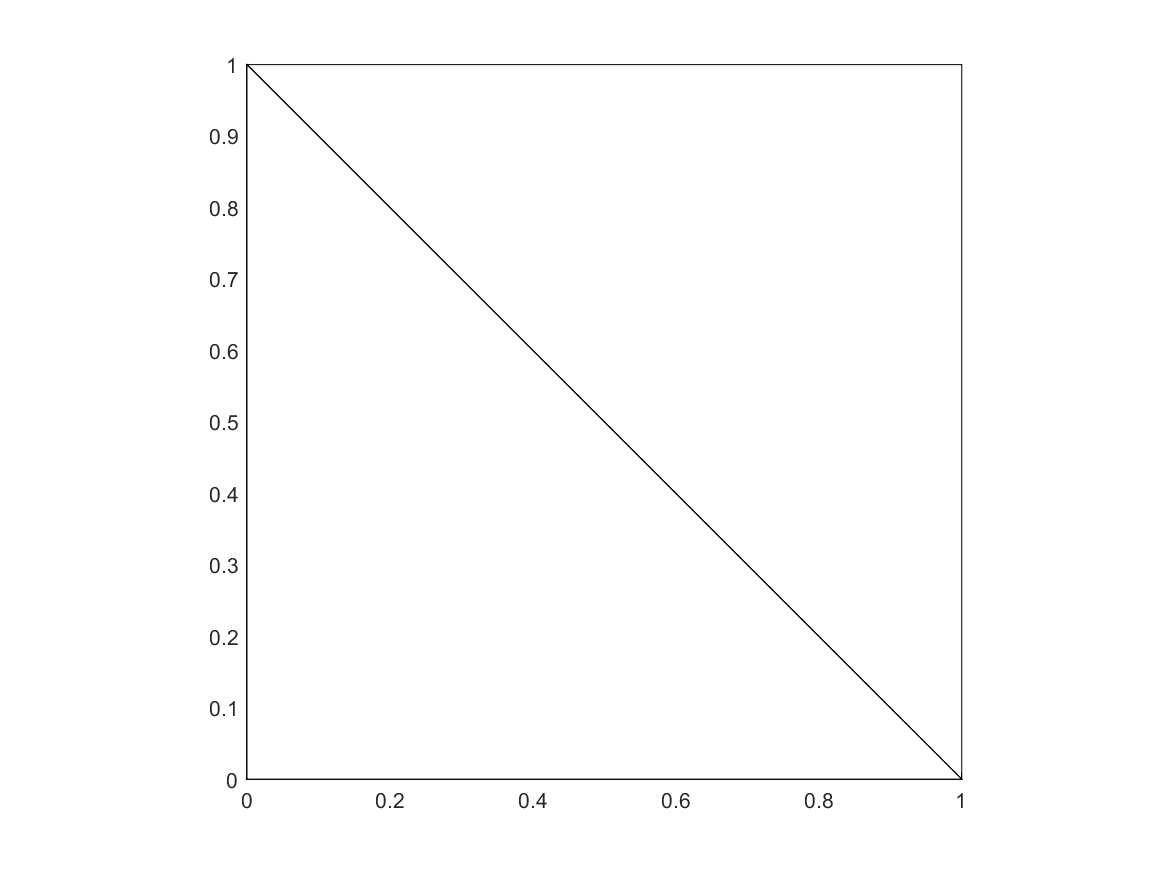
\includegraphics[trim = 90 30 90 20, clip, width=\linewidth]
      {pictures/chapExperiments/secGeneralInfo/squareTriang.png}
    \label{fig:triangSquare}
  \end{subfigure}
  \caption{In den Experimenten genutzte initiale Triangulierungen.}
  \label{fig:initialTriangulations}
\end{figure}
Führen wir ein Experiment mit adaptiver Netzverfeinerung durch, so wählen wir
den Bulk-Parameter für den Mark-Schritt des AFEM-Algorithmus $\theta=0.5$ und
den Parameter $\gamma=1$ für den Verfeinerungsindikator aus 
\Cref{def:refinementIndicator}.
Außerdem betrachten wir zur Wahl des Parameters $\gamma$ auf dem
Verfeinerungsindikator in \Cref{sec:experimentsWithExactSolution} ein
Experiment.
Auf die Wahl der Parameter $\tau$ und $\epsstop$ für die primale-duale
Iteration werden wir im folgenden \Cref{sec:choiceOfParameters} eingehen.
Die maximale Iterationszahl ist, mit Ausnahme von einem Experimente in
\Cref{sec:choiceOfParameters}, mit $10^{12}$ so gewählt, dass diese nie 
der Grund für das Beenden einer primalen-dualen Iteration ist, also stets das
Abbruchkriterium aus \eqref{eq:terminationCriterion} für den Abbruch
verantwortlich ist.
Die minimale Anzahl der Freiheitsgrade ist so gewählt, dass AFEM-Routine
manuell oder durch Server beendet wird, bevor Sie durch erreichen 
der Freiheitsgrade beendet wird. Dies geschah in allen Experimenten bei 
ungefähr $10^6$ Freiheitsgraden.

\begin{table}[p]
  \centering
  \begin{tabular}{c|c}
    \hline
    \texttt{benchmark} & Abbildungen\\  
    \hline 
    \texttt{denoiseAlpha100} &
    \ref{fig:snr15alpha100}\\
    \texttt{denoiseAlpha1000} &
    \ref{fig:snr15alpha1000}\\
    \texttt{denoiseAlpha2500} &
    \ref{fig:snr15alpha2500}\\
    \texttt{denoiseAlpha5000} &
    \ref{fig:snr15alpha5000}\\
    \texttt{denoiseAlpha10000} &
    \ref{fig:snr15alpha10000}\\
    \texttt{denoiseAlpha50000} &
    \ref{fig:snr15alpha50000}\\
    \texttt{paramsTau\_f01\_0Dot1} &
    \ref{fig:parTauMiscF}, \ref{fig:parTauConvergence},
    \ref{fig:iterationEnergyOscillations}\\
    \texttt{paramsTau\_f01\_0Dot5} &
    \ref{fig:parTauMiscF}, \ref{fig:parTauConvergence}\\
    \texttt{standard\_f01} &
    \ref{fig:parTauMiscF}, \ref{fig:parTauConvergence}, 
    \ref{fig:iterationEnergyLevel}, \ref{fig:iterationTermination},
    \ref{fig:f01Convergence}, \ref{fig:f01SolAdaptive},
    \ref{fig:f01SupplementaryInfo}, \ref{fig:parGammaConvergence},
    \ref{fig:gamma1Triang}, \ref{fig:inSiNrIterComparison}\\
    \texttt{paramsTau\_cameraman\_0Dot1} &
    \ref{fig:parTauMiscCam}\\
    \texttt{paramsTau\_cameraman\_0Dot5} &
    \ref{fig:parTauMiscCam} \\
    \texttt{standard\_cameraman} &
    \ref{fig:parTauMiscCam}, \ref{fig:camConvergence}, \ref{fig:camTriang}\\
    \texttt{noTerminationTau\_maxIter1e5} &
    \ref{fig:parTauNoConvergence}\\
    \texttt{paramsEpsStop\_1em2} &
    \ref{fig:parEpsStopConvergence}\\
    \texttt{paramsEpsStop\_1em3} &
    \ref{fig:parEpsStopConvergence}\\
    \texttt{paramsEpsStop\_1em4} &
    \ref{fig:parEpsStopConvergence}\\
    \texttt{paramsEpsStop\_1em5} &
    \ref{fig:parEpsStopConvergence}\\
    \texttt{standardUniform\_f01} &
    \ref{fig:f01Convergence}, \ref{fig:f01SupplementaryInfo}\\
    \texttt{standard\_f01Alpha1e4} &
    \ref{fig:f01LargeAlphaConvergence}, \ref{fig:inSiNrIterComparison}\\
    \texttt{standardUniform\_f01Alpha1e4} &
    \ref{fig:f01LargeAlphaConvergence}\\
    \texttt{parGamma\_0} &
    \ref{fig:parGammaConvergence}, \ref{fig:gamma0Triang}\\
    \texttt{parGamma\_0Dot5} &
    \ref{fig:parGammaConvergence}, \ref{fig:gammaDot5Triang}\\
    \texttt{standard\_f04} &
    \ref{fig:f04Convergence}, \ref{fig:inSiNrIterComparison}\\
    \texttt{standardUniform\_f04} &
    \ref{fig:f04Convergence}\\
    \texttt{standardUniform\_cameraman} &
    \ref{fig:camConvergence}\\
    \texttt{circleContinuousAdaptive} &
    \ref{fig:circConvAdaptive}, \ref{fig:circContConvergence},
    \ref{fig:circContLvl17Triang}, \ref{fig:circContFinalTriang},
    \ref{fig:circContSol}, \ref{fig:circContSolAxis}\\
    \texttt{circleDiscontinuousAdaptive} &
    \ref{fig:circConvAdaptive}\\
    \texttt{circleContinuousUniform} &
    \ref{fig:circConvUniform}, \ref{fig:circContConvergence},
    \ref{fig:circDiscLvl17Triang}, \ref{fig:circDiscFinalTriang},
    \ref{fig:circDiscSol}, \ref{fig:circDiscSolAxis}\\
    \texttt{circleDiscontinuousUniform} &
    \ref{fig:circConvUniform}\\
    \hline
  \end{tabular}
  \caption{Eingabe \texttt{benchmark} für \texttt{startAlgorithmCR} und die
  Abbildungen, die auf den Ergebnissen des jeweiligen Experiments basieren}
  \label{tab:usedBenchmarks}
\end{table} 


\section{Wahl der Parameter für die primale-duale Iteration}
\label{sec:choiceOfParameters}

Die Experimente in diesem Abschnitt zur Ermittelung der Einstellungen
für die primale-duale Iteration werden adaptiv durchgeführt und alle hier
nicht aufgeführten Parameter werden gewählt wie im vorhergehenden Abschnitt
beschrieben.
Die Eingangssignale für die Experimente sind in der Beschreibung der 
entsprechenden Abbildung angegeben.

Zunächst interessiert und die Wahl des Parameters $\tau$ in 
\Cref{alg:primalDualIteration}. 
Diesen müssen wir nach \Cref{thm:convergenceIteration} in $(0,1]$ wählen, um
Konvergenz der primalen-dualen Iteration zu garantieren.
Der Parameter $\epsstop$ wird mit $10^{-4}$ gewählt. 
Diese Wahl wird anschließend in diesem Abschnitt ebenfalls nochmal näher
betrachtet. 
\begin{figure}[p]
  \centering
  \begin{subfigure}[b]{.48\linewidth}
    \caption{Eingangssignal $f$}
    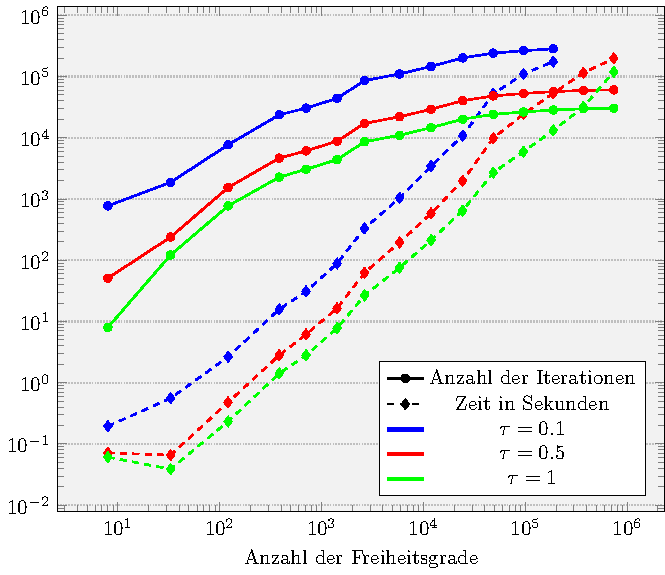
\includegraphics[width=\linewidth]
      {pictures/chapExperiments/secParameters/parTau/f01/miscF.pdf}
    \label{fig:parTauMiscF}
  \end{subfigure}
  \quad
  \begin{subfigure}[b]{.48\linewidth}
    \centering
    \caption{Eingangssignal \texttt{cameraman}}
    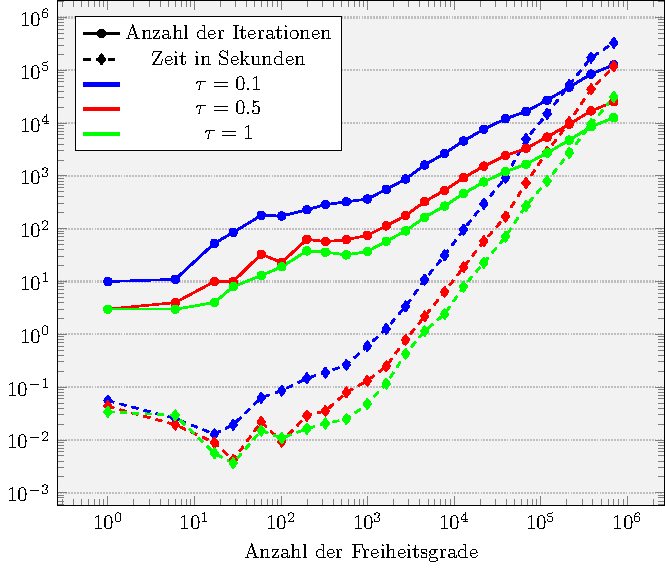
\includegraphics[width=\linewidth]
      {pictures/chapExperiments/secParameters/parTau/cam/miscCam.pdf}
    \label{fig:parTauMiscCam}
  \end{subfigure}
  \caption{Anzahl der Iterationen und benötigte Zeit für verschiedene Werte
  von $\tau$ mit den Eingangssignalen $f$ und \texttt{cameraman}.}
  \label{fig:parTauMisc}
\end{figure}
\begin{figure}[p]
  \centering
  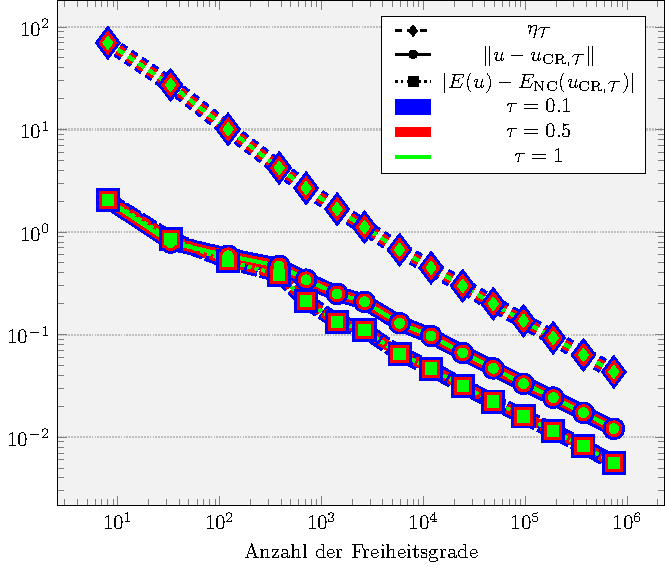
\includegraphics[width=\linewidth]
    {pictures/chapExperiments/secParameters/parTau/f01/convergenceF.pdf}
  \caption{Verfeinerungsindikator, exakter $L^2$-Fehler und Energiedifferenz 
  für verschieden Werte von $\tau$ mit Eingangangssignal $f$.}
  \label{fig:parTauConvergence}
\end{figure}
Wie in \Cref{fig:parTauMisc} zu sehen, verhält sich die Anzahl der Iteration,
und damit, wie zu erwarten war, auch die Laufzeit, antiproportional zur Größe
der hier gewählten Werte von $\tau$, d.h. größeres $\tau$ führt zu einer
geringeren Laufzeit und weniger Iterationen.
Da sich die betrachteten Graphen in \Cref{fig:parTauConvergence} für die
verschiedenen Wahlen von $\tau$ nicht sichtbar unterscheiden, schlussfolgern
wir, dass die ideale Wahl für $\tau$, die \Cref{thm:convergenceIteration}
zulässt, das heißt $\tau=1$, zu sein scheint, da die primale-duale Iteration
bei gleichen Ergebnissen für dieses $\tau$ die geringste Laufzeit hat.
Ein mögliche Erklärung liefert der Beweis von \Cref{thm:convergenceIteration}.
Die darin bewiesene \Cref{eq:upperBoundIterationError} impliziert für die
Iterate $(u_j)_{j\in\Nbb}$ auf einem Level, dass
\begin{align}
  \label{eq:nrIterationsInequality}
  \sum_{j=1}^\infty\Vert \ucrt - u_j \Vert^2 
  \leq
  \frac{1}{2\alpha\tau}
  \left(\vvvert \ucrt - u_0\vvvert^2_\nc 
  + \left\Vert \bar\Lambda_{0,\Tcal} - \Lambda_0\right\Vert^2\right)\!. 
\end{align}
Die rechte Seite ist antiproportional zu $\tau>0$, womit womöglich
die Folge $(\left\Vert \ucr - u_j\right\Vert)_{j\in\Nbb}$ schneller gegen $0$
konvergiert und damit auch das Abbruchkriterium \eqref{eq:terminationCriterion}
nach einer geringeren Anzahl von Iterationen erfüllt ist. 
Der Beweis von \Cref{thm:convergenceIteration} liefert uns keine
Informationen darüber, ob möglicherweise auch eine Wahl $\tau>1$ immer noch die
Konvergenz der primalen-dualen Iteration garantiert.
Wie aber in \Cref{fig:parTauNoConvergence} zu sehen, haben wir schon für
$\tau=1.2$ ein Beispiel gefunden, bei dem nicht davon ausgegangen werden kann,
dass die primale-duale Iteration konvergiert.
Diese Iteration wurde auf der Triangulierung aus \Cref{fig:triangBigSquare} 
durchgeführt. 
Dabei wurde die Iteration nach $10^5$ Iterationen, wie in
\Cref{fig:parTauNoConvergenceUpdates} zu sehen, abgebrochen, da kein anderes
Verhalten mehr zu erwarten war, zumal selbst für die nach
\Cref{fig:parTauMiscF} suboptimale Wahl $0.1$ für $\tau$ weniger also $10^3$
Iterationen auf der gleichen Triangulierung benötigt wurden und für die Wahl
$\tau=1$ sogar weniger als $10$ Iterationen.
\begin{figure}[p]
  \centering
  \begin{subfigure}[b]{.48\linewidth}
    \centering
    \caption{Mussugen der Updates}
    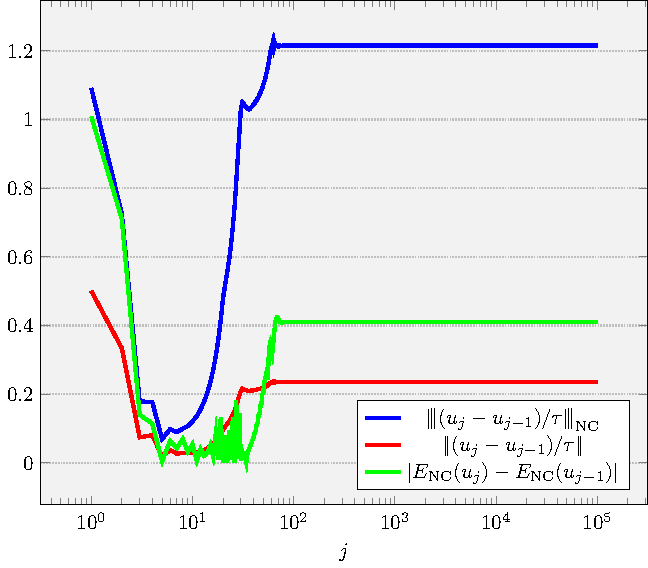
\includegraphics[width=\linewidth]
      {pictures/chapExperiments/secParameters/parTau/f01NoConv/1Dot2/convIter.pdf}
    \label{fig:parTauNoConvergenceUpdates}
  \end{subfigure}
  \quad
  \begin{subfigure}[b]{.47\linewidth}
    \centering
    \caption{Verlauf der Energie}
    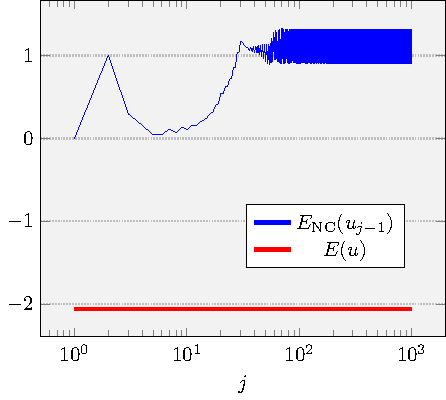
\includegraphics[width=\linewidth]
      {pictures/chapExperiments/secParameters/parTau/f01NoConv/1Dot2/convEnergy.pdf}
    \label{fig:parTauNoConvergenceEnergy}
  \end{subfigure}
  \caption{Drei Messungen des Updates der Iteration (a) und Verlauf der
  Energie während der erstens $1000$ Iterationen (b) für $\tau=1.2$ mit
  Eingangangssignal $f$.}
  \label{fig:parTauNoConvergence}
\end{figure}
Auch die Betragsdifferenz zwischen den Energien zweier Iterate stagniert.
Es ist stark davon auszugehen, dass dieses Problem mit keinem von den
Iteraten abhänigen Abbruchkriterium terminiert.
Mit \Cref{fig:parTauNoConvergenceEnergy} steht außerdem fest, dass der
Abstand zwischen den Iteraten nicht stagniert, während die Iterate divergieren
oder konvergieren, sondern dass die Iterate sich mit alternierender Energie
entwickeln zu scheinen.
Insbesondere bleibt festzuhalten, dass die von \Cref{thm:convergenceIteration}
für $\tau\in(0,1]$ garantierte Konvergenz für $\tau=1.2$ nicht eintritt.

Nun betrachen wir die Wahl des Parameteres $\epsstop$ für das Abbruchkriterium
aus \eqref{eq:terminationCriterion}.
\begin{figure}[p]
  \centering
  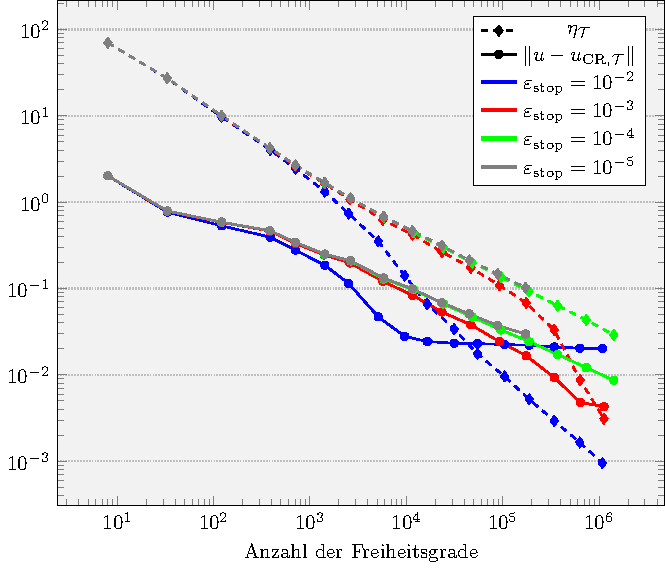
\includegraphics[width=\linewidth]
    {pictures/chapExperiments/secParameters/parEpsStop/f01/convergenceF.pdf}
  \caption{Verfeinerungsindikator und exakter $L^2$-Fehler für verschieden
  Werte von $\epsstop$ mit Eingangangssignal $f$.}
  \label{fig:parEpsStopConvergence}
\end{figure}
Wie in \Cref{fig:parEpsStopConvergence} zu sehen, stagniert der 
exakte $L^2$-Fehler für $\epsstop=10^{-2}$ und, es lässt sich erahnen, dass
dieser Effekt auch für $\epsstop=10^{-3}$ einsetzt. 
Da der Effekt bis $10^6$ Freiheitsgrade für $\epsstop\in\{10^{-4},10^{-5}\}$
noch nicht einsetzt, scheint dies an einem zu frühen Abbruch der Iteration 
durch eine zu große Toleranz $\epsstop$ zu liegen. 
Bei hohen Freiheitsgraden und einer entsprechend kleinen Netzweite muss
also $\epsstop$ ausreichend klein gewählt werden.
Da wir in den Experimenten  $10^6$ Freiheitsgrade nicht deutlich überschreiten
und sich bis dahin die Ergebnisse für die Wahlen $10^{-4}$ und $10^{-5}$ kaum
unterscheiden, die Wahl $10^{-5}$ aber eine wesentlich längere Laufzeit
verursacht, wählen wir als Standard $\epsstop=10^{-4}$.
Weiterhin bleibt festzuhalten, dass der Verfeinerungsindikator trotzdem noch
passend Dreiecke auswählt und weiter fällt, d.h. insbesondere nicht
stagnariert, auch bei stagnierendem Fehler.


\section{Experimente mit bekannter exakter Lösung}
\label{sec:experimentsWithExactSolution}

In diesem Abschnitt möchten wir nun anhand des Experiments mit Eingangssignal
$f_1$ aus \Cref{eq:inputSignalF01} die Ergebnisse des Programms betrachten.
Außerdem werden wir die Ergebnisse mit zwei weiteren Eingangssignalen,
für die exakte Lösungen bekannt sind, vergleichen, um so weitere Aussagen
über die Ergebnisse treffen zu können.
Die Wahl aller Parameter, die hier nicht noch einmal aufgeführt werden, ist
im einleitenden Teil und dem vorherigen \Cref{sec:choiceOfParameters} 
begründet worden.

\DTLloaddb{db}{data/currentDataReducedParTau1em1Lvl1.csv}
\DTLassign{db}{1}{\nrDof=nrDof} 
\DTLgdeletedb{db}
Zunächst möchten wir anhand der Experimente mit Eingangssignal $f_1$ einige
Eigenschaften der primalen-dualen Iteration betrachten.
\begin{figure}[p]
  \centering
  \begin{subfigure}[b]{.5\linewidth}
    \centering
    \caption{Energieverlauf der Iterationen per Level}
    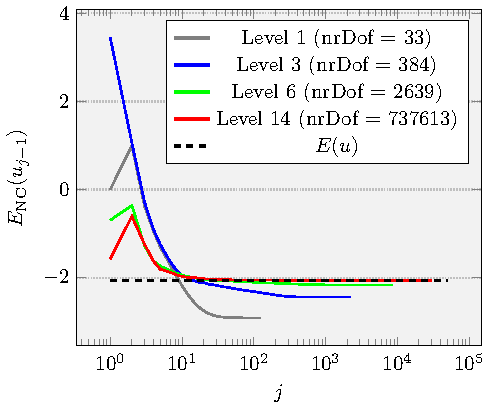
\includegraphics[width=\linewidth]
      {pictures/chapExperiments/secExactSol/iteration/lvlWise/convEnergy.pdf}
    \label{fig:iterationEnergyLevel}
  \end{subfigure}
  \quad
  \begin{subfigure}[b]{.46\linewidth}
    \centering
    \caption{Oszillierendes Beispiel}
    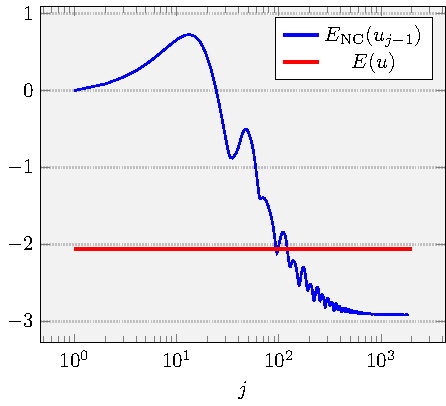
\includegraphics[width=\linewidth]
      {pictures/chapExperiments/secExactSol/iteration/osc/convEnergy.pdf}
    \label{fig:iterationEnergyOscillations}
  \end{subfigure}
  \caption{Energieentwicklung während der primalen-dualen Iteration für
  Eingangssignal $f$ auf verschiedenen Leveln mit $\tau=1$ (a) und für ein
  Level mit $\tau=10^{-1}$ (b) wobei das initale Level 0 ist.}
  \label{fig:iterationEnergy}
\end{figure}
In \Cref{fig:iterationEnergyLevel} sehen wir an einer Auswahl von Leveln der
AFEM-Routine, wobei das erste Level mit 0 nummeriert wird, dass die
nichtkonforme Energie $\Enc(\bullet)$ der Iterate von oben konvergiert. 
Dabei nimmt der Abstand zu der Energie der exakten Lösung
$E(u)$ mit zunehmender Anzahl von Freiheitsgraden ab.
Anhand der Energieentwicklung des ersten Iterationsschritt aller abgebildeten
Level, mit Ausnahme von Level 3, und insbesondere durch
\Cref{fig:iterationEnergyOscillations}, die auf dem gleichen Experiment mit
$\tau=10^{-1}$ basiert und Level 1 dieses Experiments mit \nrDof\ 
Freiheitsgraden, ist aber auch klar erkennbar, dass die Energie der Iterate
nicht monoton fallend von oben konvergiert.
Dieses Verhalten könnte mit ein Grund dafür sein, dass die Anzahl der 
Iterationen, wie schon in \Cref{fig:parTauMiscF} gesehen, bei kleinem
$\tau=10^{-1}$ deutlich höher ist als bei $\tau=1$.
\begin{figure}[p]
  \centering
  \begin{subfigure}[b]{.5\linewidth}
    \centering
    \caption{Updatenorm per Level}
    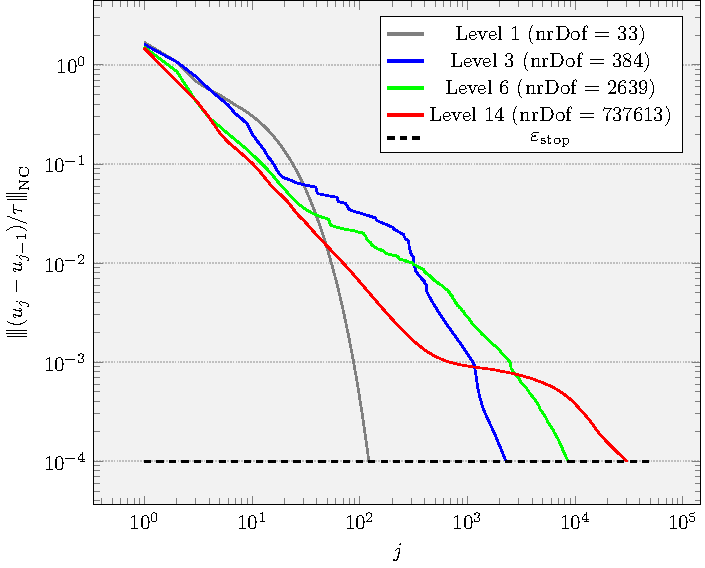
\includegraphics[width=\linewidth]
      {pictures/chapExperiments/secExactSol/iteration/lvlWise/termLvl.pdf}
    \label{fig:iterationLevel}
  \end{subfigure}
  \quad
  \begin{subfigure}[b]{.46\linewidth}
    \centering
    \caption{verschiedene mögliche Abbruchkriterien}
    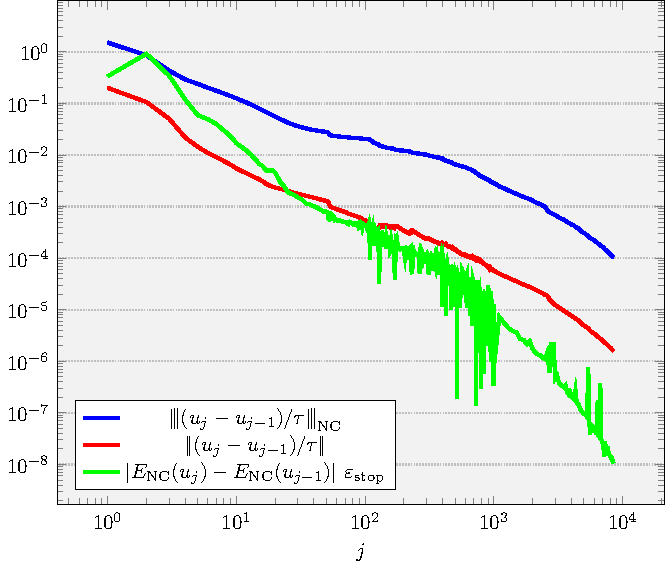
\includegraphics[width=\linewidth]
      {pictures/chapExperiments/secExactSol/iteration/lvlWise/termComp.pdf}
    \label{fig:iterationTerminationVariants}
  \end{subfigure}
  \caption{Abbruchkriterien wobei das initiale Level 0 ist.}
  \label{fig:iterationTermination}
\end{figure}
In \Cref{fig:iterationLevel} ist dann noch die Entwicklung des für die 
Abbruchbedingung relevanten Terms für verschieden Level zu sehen, der wie
gewünscht fällt bis die Toleranz erreicht ist.
Zusätzlich sind in \Cref{fig:iterationTerminationVariants} von Level 6 des
gleichen Experiments die Verläufe zweier weiterer Terme zu sehen, die 
man für Abbruchkriterien bedenken könnte, da ihre Konvergenz gegen $0$ erwartet
ist. 
Dabei unterscheidet sich der Term, der sich lediglich in der Norm
unterscheidet, nur um einen Faktor von ungefähr $10^2$. 
Dies passt zur bekannten Theorie, da die Norm
$\vvvert\bullet\vvvert_\NC$ ungefähr so skaliert wie $h^{-1}\Vert\bullet\Vert$
(cf. inverse Ungleichung \cite[Lemma 3.5]{Bar15}, diskrete
Poincar\'e-Ungleichung \cite[Lemma 3.7]{Bar15}), wobei für dieses Level
$h\approx 10^{-2}$ .
Entsprechend müsste man nur, bei Wahl dieses Abbruchkriteriums, die Toleranz 
entsprechend kleiner wählen.
Die Differenz der nichtkonformen Energien zweiter Iterate scheint sich aber,
aufgrund der teils starken Oszillationen, nur schlecht als alternatives
Abbruchkriterium zu eignen, obwohl sie wie erwartet gegen $0$ konvergieren.

Nun betrachten wir Konvergenzraten und überprüfen die Gültigkeit einiger in den
theoretischen Kapiteln dieser Arbeit getätigten Aussagen.
\begin{figure}[p]
  \centering
  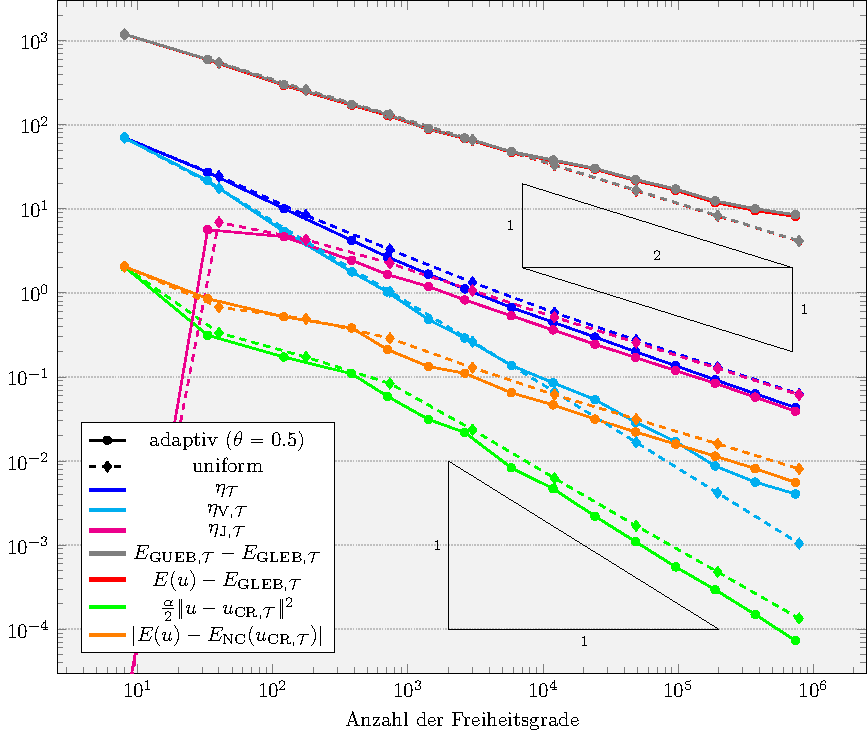
\includegraphics[width=\linewidth]
    {pictures/chapExperiments/secExactSol/f01/conv.pdf}
  \caption{Ergebnisse der adaptiven und uniformen AFEM-Schleifen für das 
  Eingangssignal $f$.}
  \label{fig:f01Convergence}
\end{figure}
\begin{figure}[p]
  \DTLloaddb{db}{data/currentDataReducedStandardF01LvlFinal.csv}
  \DTLassign{db}{1}{\nrDof=nrDof} 
  \DTLgdeletedb{db}
  \centering
  \begin{subfigure}[b]{.48\linewidth}
    \centering
    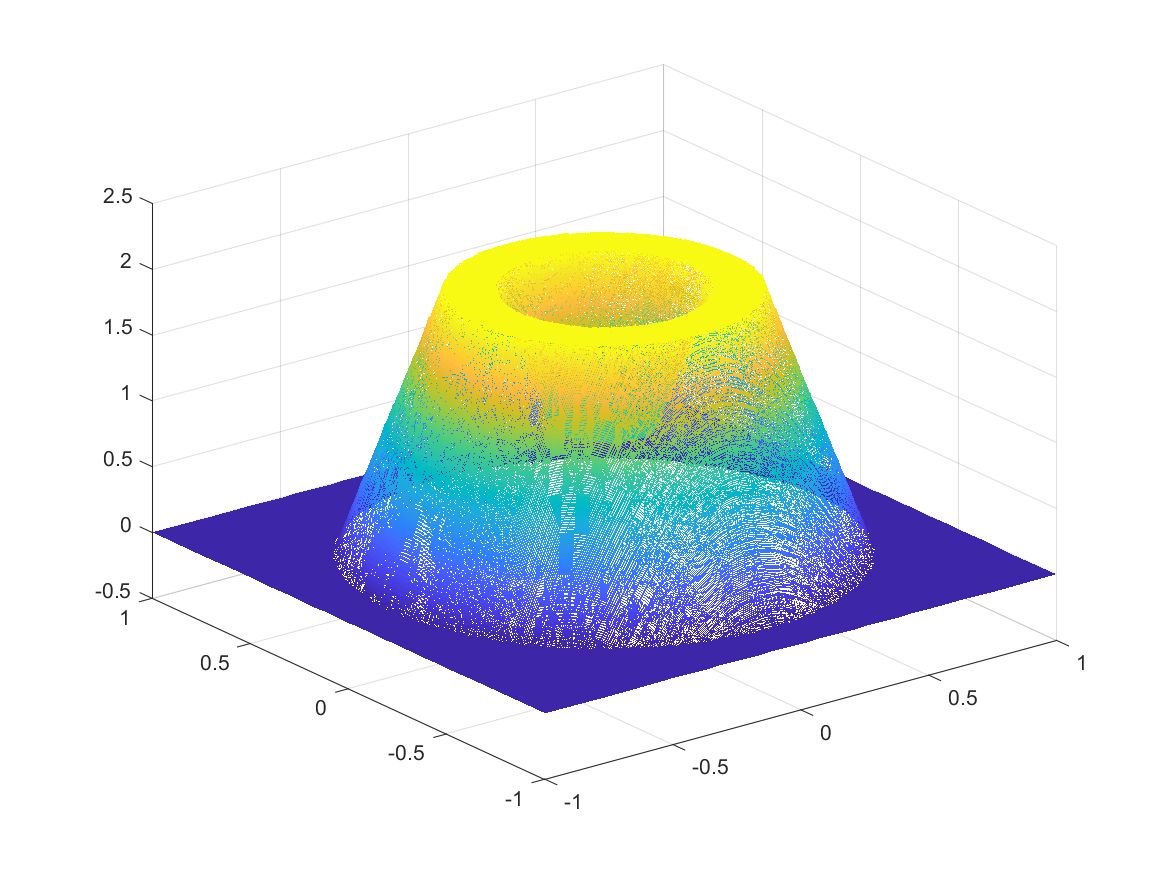
\includegraphics[trim = 40 30 30 30, clip, width=\linewidth]
      {pictures/chapExperiments/secExactSol/f01/adaptive/lvl14/solution.png}
    \label{fig:f01SolAdaptivePlot}
  \end{subfigure}
  \quad
  \begin{subfigure}[b]{.48\linewidth}
    \centering
    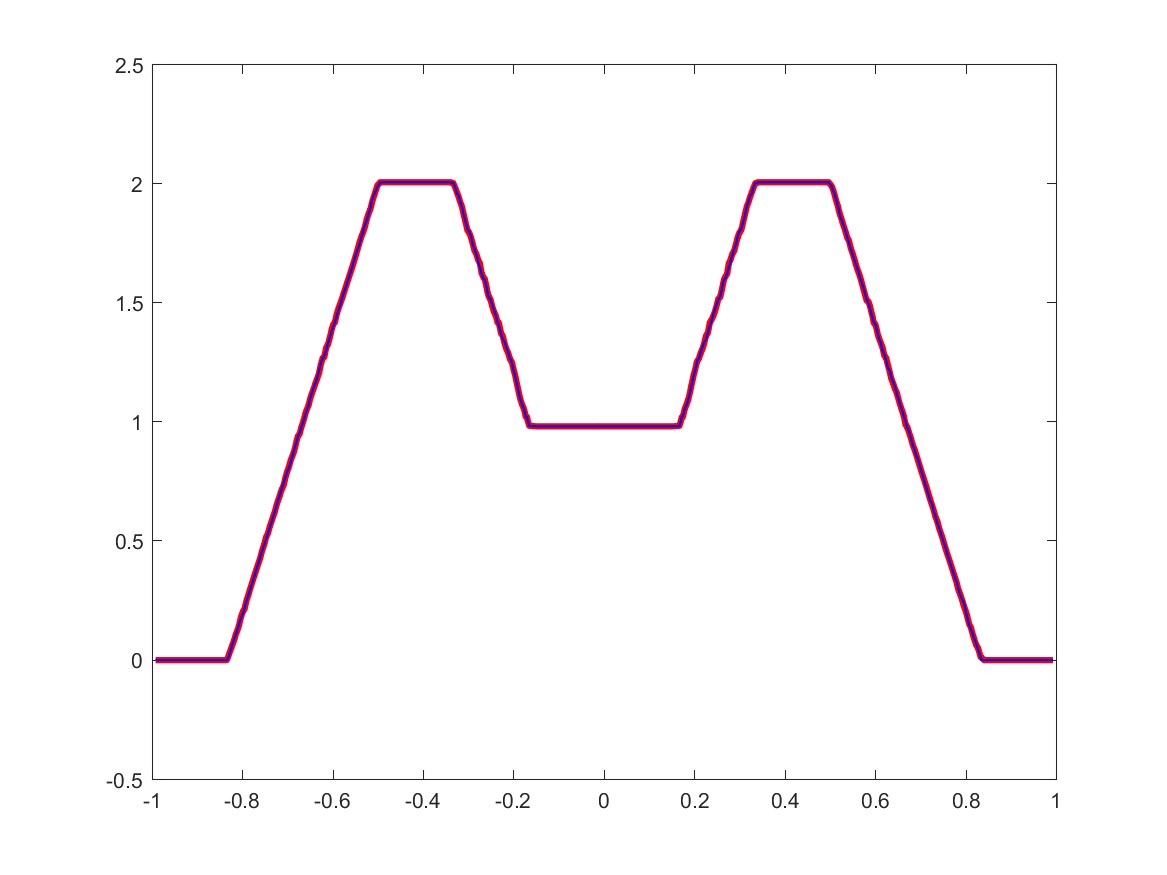
\includegraphics[trim = 50 30 50 20, clip, width=\linewidth]
      {pictures/chapExperiments/secExactSol/f01/adaptive/lvl14/solutionAxis.png}
    \label{fig:f01SolAdaptiveAxis}
  \end{subfigure}
  \caption{Lösung des adaptiven Algorithmus mit Eingangssignale $f$ sowie deren
  Darstellungen entlang der x-Achse (blau) und der y-Achse (rot) auf einem
  Gitter mit \nrDof\ Freiheitsgraden.}
  \label{fig:f01SolAdaptive}
\end{figure}
\begin{figure}[p]
  \centering
  \begin{subfigure}[b]{.48\linewidth}
    \centering
    \caption{Unterschiede oberer beiden Graphen}
    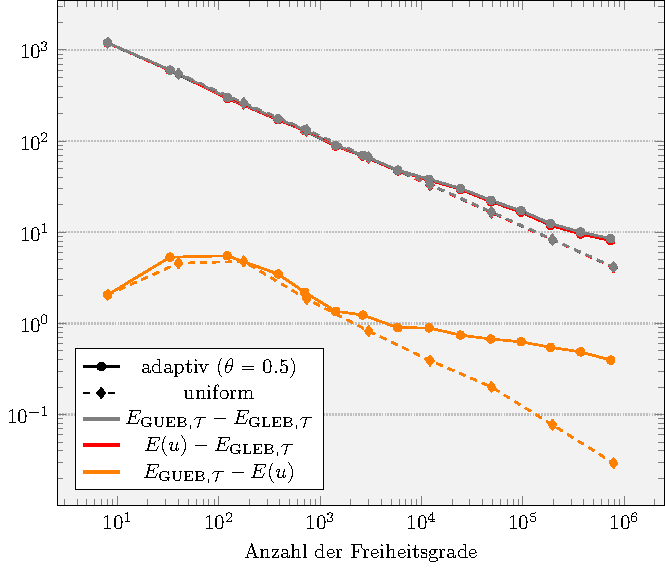
\includegraphics[width=\linewidth]
      {pictures/chapExperiments/secExactSol/f01/energyDiffs.pdf}
    \label{fig:f01DiffGuebExactE}
  \end{subfigure}
  \quad
  \begin{subfigure}[b]{.48\linewidth}
    \centering
    \caption{Sprungterm Entwicklung}
    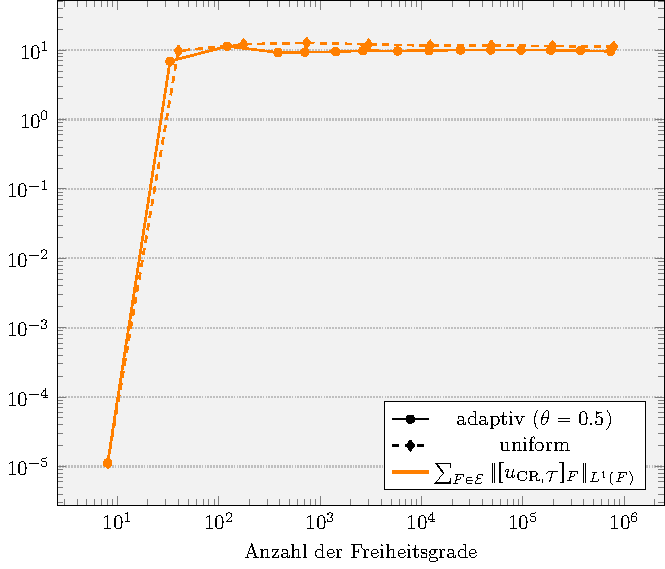
\includegraphics[width=\linewidth]
      {pictures/chapExperiments/secExactSol/f01/jumpTerms.pdf}
    \label{fig:f01JumpTerms}
  \end{subfigure}
  \caption{Zusätzliche Infos für Eingangangssignal $f$.}
  \label{fig:f01SupplementaryInfo}
\end{figure}
Wie in \Cref{fig:f01Convergence} zu sehen, unterscheiden sich die Raten für
uniforme und adaptive Netzverfeinerungen für das Eingangssignal $f_1$ nicht.
Alle Graphen konvergieren mit einer Rate von etwa $1/2$ mit Ausnahme
des quadrierten exakten Fehlers und dem Volumenanteil des Fehlerschätzers,
die mit einer Rate von ungefähr $1$ konvergieren.
Nach \cite[S. 309, Theorem 10.7]{Bar15} erwarten wir für die von Professor
Bartels betrachtete Version des Problem, das heißt der Diskretisierung mit
dem Courant-Finite-Elemente-Raum $S^1(\Tcal)$, für den quadrierten $L^2$-Fehler
zwischen den Minimierern $u_\C\in S^1(\Tcal)$ und $u\in\BV(\Omega)\cap
L^2(\Omega)$ des Funktionals $I$ aus \Cref{eq:rofModel} in den entsprechenden
Räumen, eine entsprechend Rate von mindestens $1/4$, welche für seine
Problemstellung garantiert ist.
Obwohl wir eine andere Formulierung des ROF-Modells betrachten, können
wir festhalten, dass wir diese Rate deutlich überschreiten, unser 
Programm in diesem Setting also nicht schlechter ist als die garantierte 
Rate der anderen Formulierung.
Dabei bleibt aber noch hervorzuheben, dass gilt 
$u_1,f_1\in H^1_0\left( (0,1)^2 \right)$, wir also ein reguläreres Problem
betrachten als eines, in dem die exakte Lösung nur eine $\BV$-Funktion ist
und nicht schwach differenzierbar.
Insofern ist die deutlich bessere Rate so zu erwarten gewesen.
Wir werden deshalb am Ende dieses Abschnitts ein noch regulärer Problem
betrachten und untersuchen, ob dies die Raten noch weiter verbessern kann.
Als nächstes gilt nach \Cref{fig:f01Convergence}, dass
\begin{align}
  \label{eq:expectedInequalities}
  \frac{\alpha}{2}\Vert u -\ucrt\Vert^2
  \leq
  E(u)-\Egleb
  \leq
  \Egueb-\Egleb,
\end{align}
wie wir nach \Cref{thm:gleb} und Ungleichung \ref{eq:gueb} erwartet haben.
Dabei merken wir an, dass dieser Sachverhalt für $E(u)-\Egleb\leq\Egueb-\Egleb$
nur schwer zu erkennen ist, aber gilt, wie dank \Cref{fig:f01DiffGuebExactE} zu
sehen ist, da $\Egueb-\Egleb-(E(u)-\Egleb) = \Egueb-E(u)$.
In \Cref{fig:f01JumpTerms} sehen wir weiterhin, dass die Sprungterme in
unserere nichtkonformen Formulierung tatsächlich nicht minimiert werden. 
Zwar sind die jeweiligen Sprünge zwischen zwei Dreiecken bei einer hohen Anzahl
von Freiheitsgraden klein, wie \Cref{fig:f01SolAdaptive} erahnen lässt, jedoch
wird durch die hohe Anzahl von Kanten eine große Menge von kleinen Sprüngen
addiert, die zu einer relativ großen Summe führen.
Da durch \Cref{fig:f01Convergence} zu sehen ist, dass $|E(u)-\Enc(\ucrt)|$
konvergiert, wird insgesamt klar, dass $E(\ucrt)$, im Gegensatz zu
$\Enc(\ucrt)$, nicht gegen $E(u)$ konvergiert, wie zu erwarten war nach der
Herleitung in \Cref{sec:discreteProblemFormulation}.
Zum Abschluss weisen wir darauf hin, dass die Konvergenz von $\Enc(\ucrt)$
gegen $E(u)$ durch betrachten von \Cref{fig:iterationEnergyLevel} bereits zu
sehen war, in der der Abstand des augenscheinlichen Grenzwerts der Iteration
mit höhrerem Level näher an $E(u)$ liegt.
Aus \Cref{fig:f01Convergence} geht auch hervor, dass der Verfeinerungsindikator
zum Schluss vom Sprunganteil dominiert wird und der Einfluss des Volumenanteils
vernachlässigbar wird.
In $\etaV$ liegt auch der deutlichste Unterschied zwischen adaptiven und
uniformen Algorithmus. Bei uniformer Netzverfeinerung erreicht $\etaV$ eine
leicht bessere Rate und geringere Werte als bei adaptiver Netzverfeinerung,
da im adaptiven Algorithmus zu den Sprüngen hin verfeinert wird, was im 
geringfügig geringeren Wert von $\etaJ$ im adaptiven Algorithmus zu sehen ist.
Da $\etaV$ geringer ist im uniformen Algorithmus, ist nach der Definition der
garantierten unteren Energieschranke in \Cref{eq:gleb} zu erwarten, dass
$\Egleb$ größere Werte annimmt, was sich in \Cref{fig:f01Convergence}
tatsächlich in den beiden Graphen widerspiegelt, in denen $\Egleb$ subtrahiert
wird, die im uniformen Algorithms geringere Werte annehmen als im adaptiven.
Durch den geringeren Wert von $\etaJ$ für den adaptiven Algorithmus und die
deutliche Dominanz dessen in $\etaT$, nimmt tatsächlich $\etaT$ im adaptiven
Algorithmus leicht geringere Werte an, trotz des Unterschieds von $\etaV$.
Nun wollen wir noch anmerken, dass aus \Cref{thm:convexity} und
\Cref{sec:discreteProblemFormulation} folgt, dass
\begin{align*}
  \frac{\alpha}{2}\Vert u-\ucrt\Vert^2\leq
  E(\ucrt)-E(u)=\Enc(\ucrt)+\sum_{F\in\Ecal}\Vert[\ucrt]_F\Vert_{L^1(F)}-E(u).
\end{align*}
Insbesondere gilt auch 
\begin{align*}
  \frac{\alpha}{2}\Vert u-\ucrt\Vert^2
  \leq
  \left|\Enc(\ucrt)-E(u)\right|+
  \sum_{F\in\Ecal}\Vert[\ucrt]_F\Vert_{L^1(F)}.
\end{align*}
Dieser Aussage widerspricht \Cref{fig:f01Convergence} nicht, obwohl die Sprünge,
die auf der rechten Seite dieser Ungleichung stehen, im Plot nicht einbezogen
sind.
Zum Abschluss dieses Experiments betonenen wir noch, dass
\Cref{fig:f01SolAdaptive} zeigt, dass das Ergebnis des adaptiven Algorithmus
tatsächlich der erwarteten exakten Lösung $u$ aus \Cref{fig:f01Plots} ähnelt.

Mit diesen Erkenntnisen betrachten wir nun noch die Wahl von $\gamma$
aus der \Cref{def:refinementIndicator} des Verfeinerungsindikators $\etaT$.
Je kleiner die Wahl von $\gamma$, desto größer sollte der Einfluss von
$\etaJ$ auf $\etaT$ sein und entsprechend eine stärkere Verfeinerung zu
den Sprüngen geschehen.
\begin{figure}[p]
  \centering
  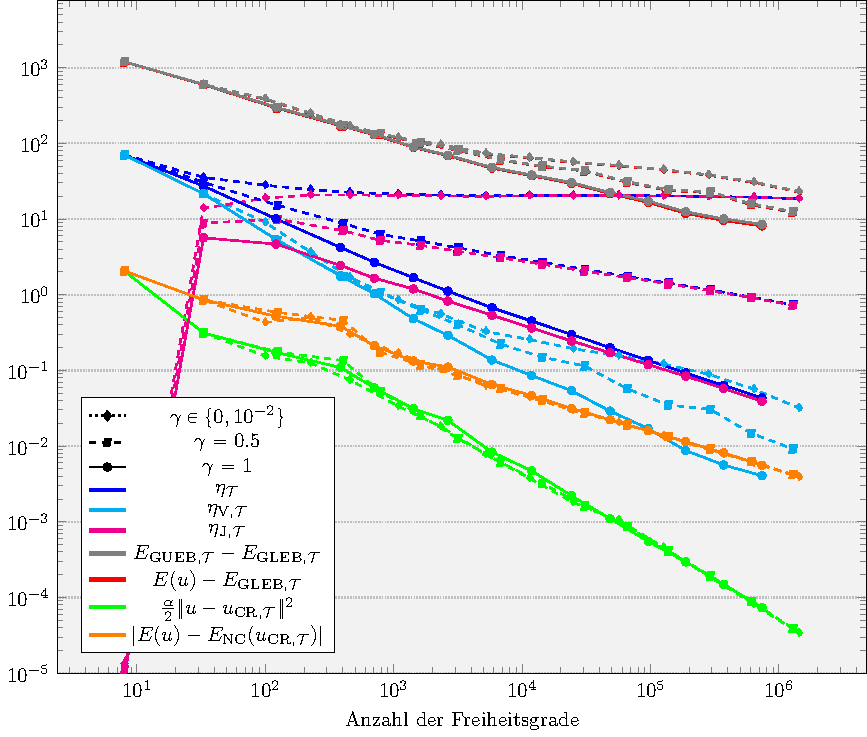
\includegraphics[width=\linewidth]
    {pictures/chapExperiments/secExactSol/parGamma/conv.pdf}
    \caption{$\gamma$ Plots, wobei die Graphen für $\gamma \in\{0,10^{-2}\}$
    nicht sichtbar unterscheidbar sind und nur der Graph für $\gamma=0$
    dargestellt ist.}
  \label{fig:parGammaConvergence}
\end{figure}
In \Cref{fig:parGammaConvergence} ist tatsächlich zu erkennen, dass
$\etaJ$ mit kleinerem $\gamma$ deutlich größere Werte annimmt. 
Tatsächlich stagniert $\etaJ$ für $\gamma=0$ sogar und entsprechend gilt 
dies auch für $\etaT$.
Da die Sprungterme $\sum_{F\in\Ecal(\Tcal)}\Vert [\ucrt]_F\Vert_{L^1(F)}$ 
im diskreten Problem nicht minimiert werden, wie in
\Cref{sec:discreteProblemFormulation} beschrieben, ist dies das Resultat davon.
Weiterhin ist $\etaV$ und damit, wie im vorherigen Experiment erklärt,
die Graphen mit $\Egueb$, entsprechend der Wahl von $\gamma$ schlechter,
wenn zu den Sprungen verfeinert wird.
Bei $\gamma=0$ wird stark zu den Sprüngen hin verfeinert, welche aber nicht
minimiert werden, womit keine Reduktion von $\etaT$ stattfindet.
Da wir im vorherigen Experiment bereits gesehen habe, dass Adaptivität die 
Konvergenzrate nicht verbessert im Vergleich zur uniformen Netzverfeinerung,
ist von der noch deutlicheren adaptive Verfeinerung zu den Sprüngen
keine Verbesserung zu erwarten gewesen.
Alle Graphen, die nicht direkt von 
$\etaV$ abhänger, für alle Wahlen von $\gamma$ gleich.
\begin{figure}[p]
  \centering
  \begin{subfigure}{.32\linewidth}
    \centering
    \DTLloaddb{db}{data/currentDataReducedParGamma0LvlFinal.csv}
    \DTLassign{db}{1}{\nrDof=nrDof} 
    \DTLgdeletedb{db}
    \caption{$\gamma=0$, $\text{nrDof}=\nrDof$}
    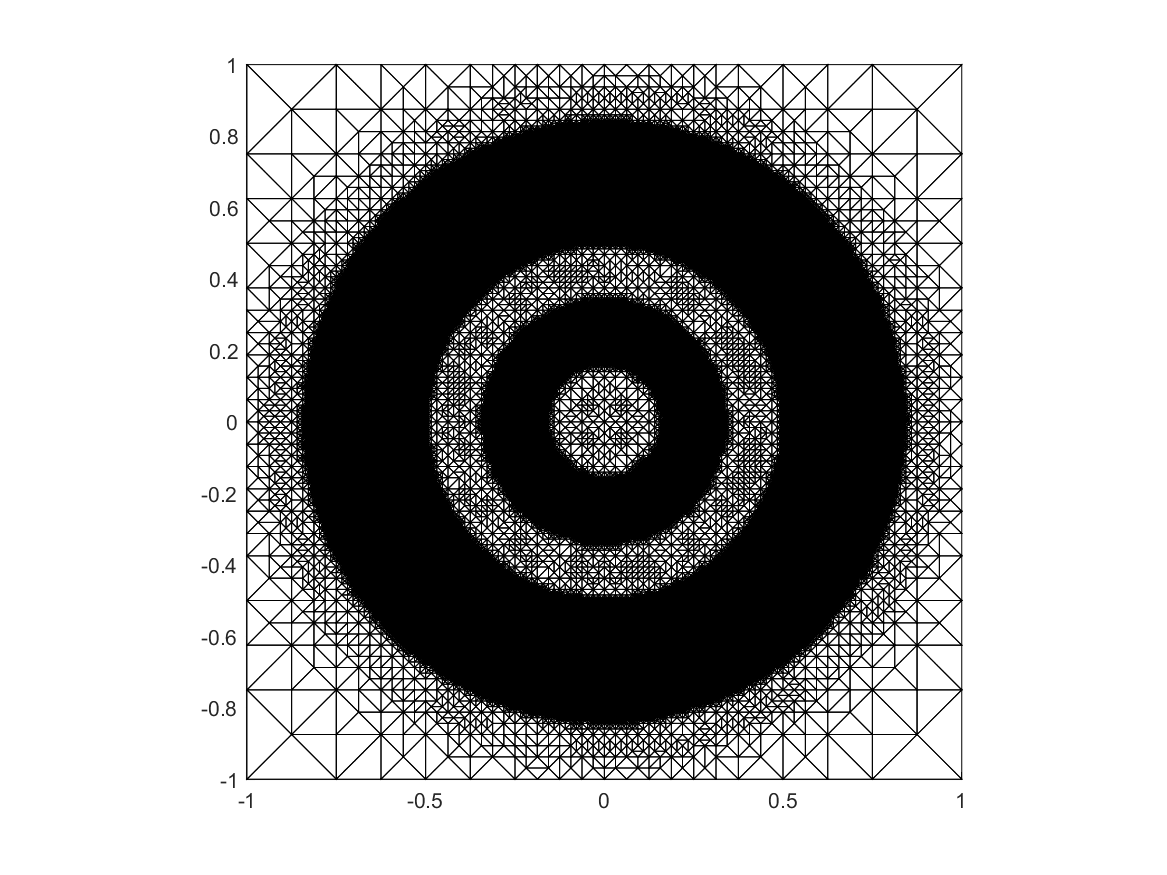
\includegraphics[trim = 100 30 80 20, clip, width=\linewidth]
      {pictures/chapExperiments/secExactSol/parGamma/0/lvl14/triangulation.png}
    \label{fig:gamma0Triang}
  \end{subfigure}
  \begin{subfigure}{.32\linewidth}
    \centering
    \DTLloaddb{db}{data/currentDataReducedParGamma5em1LvlFinal.csv}
    \DTLassign{db}{1}{\nrDof=nrDof} 
    \DTLgdeletedb{db}
    \caption{$\gamma=0.5$, $\text{nrDof}=\nrDof$}
    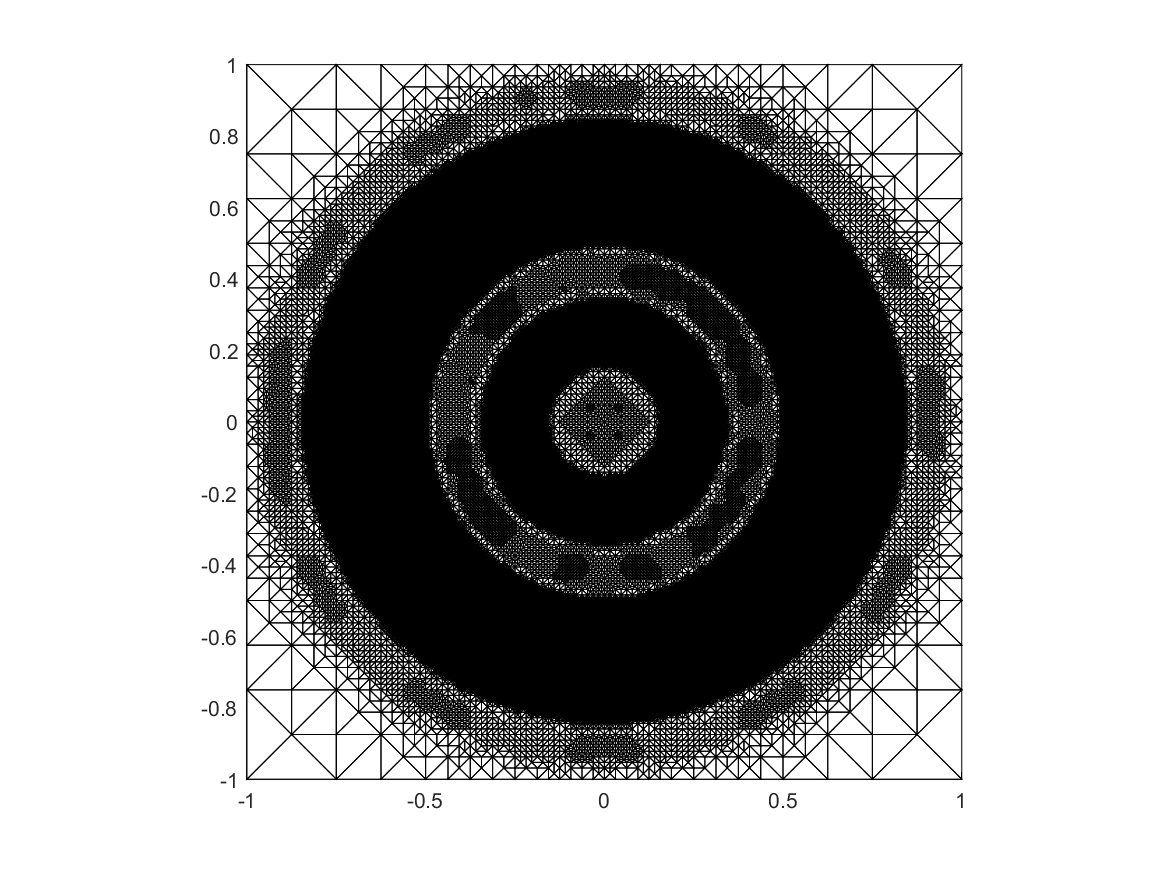
\includegraphics[trim = 100 30 80 20, clip, width=\linewidth]
      {pictures/chapExperiments/secExactSol/parGamma/5em1/lvl14/triangulation.png}
    \label{fig:gammaDot5Triang}
  \end{subfigure}
  \begin{subfigure}{.32\linewidth}
    \centering
    \DTLloaddb{db}{data/currentDataReducedStandardF01LvlFinal.csv}
    \DTLassign{db}{1}{\nrDof=nrDof} 
    \DTLgdeletedb{db}
    \caption{$\gamma=1$, $\text{nrDof}=\nrDof$}
    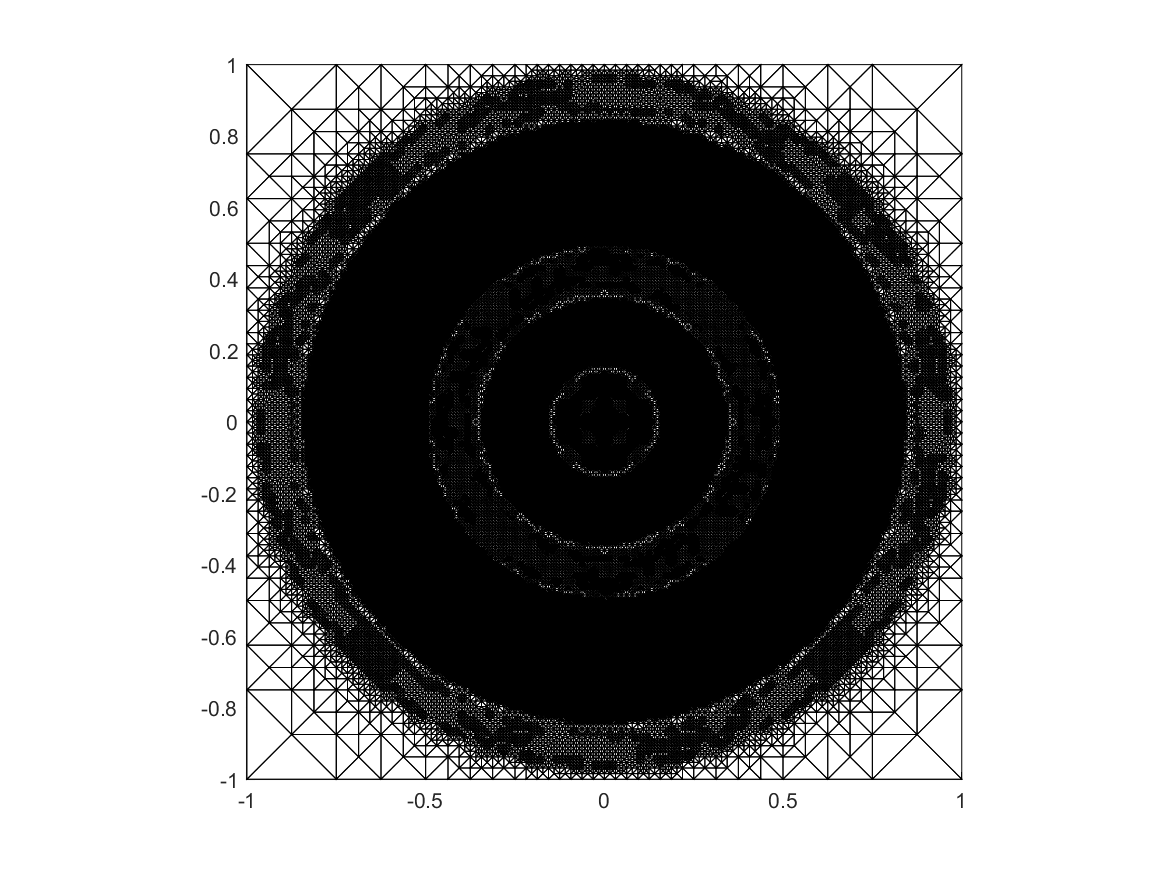
\includegraphics[trim = 100 30 80 20, clip, width=\linewidth]
      {pictures/chapExperiments/secExactSol/parGamma/1/lvl14/triangulation.png}
    \label{fig:gamma1Triang}
  \end{subfigure}
  \caption{$\gamma$ Triangulierungen Plots des jeweils letzten erreichten 
  Levels (14).}
  \label{fig:gammaTriangs}
\end{figure}
In \Cref{fig:gammaTriangs} ist die Wirkung des Verfeinerungsindikators gut zu
erkennen. 
Die Sprünge sind da am höchsten, wo die Lösung, und damit im Endeffekt die
Iterate, nicht konstant sind.   
Entsprechend wird mit kleinerem $\gamma$ stark dort verfeinert, wo die Lösung
$u$ aus \Cref{fig:f01Plots} nicht konstant ist.
Obwohl die abgebildeten Triangulierungen für kleine $\gamma$ mehr 
Freiheitsgrade hat, ist die Lokalität der Verfeinerung trotzdem stärker
als für $\gamma=1$.
Insgesamt halten wir fest, dass die zu Beginn des Kapitels getroffene Wahl
von $\gamma=1$ weiterhin sinnvoll bleibt, da so auch für den
Verfeinerungsindikator eine Konvergenz zu erkennen ist, bzw. die besten
Raten, bei keinem Einfluss auf den exakten Fehler.
Auch hier möchten wir zum Abschluss kurz anmerken, dass Ungleichung
\eqref{eq:expectedInequalities} für alle Wahlen von $\gamma$ gültig ist.

Nun wollen wir das Experiment zu \Cref{fig:f01Convergence} noch kurz mit
$\alpha=10^4$ betrachten, das heißt insbesondere mit Eingangssignal
$\alpha=10^4$.
\begin{figure}[p]
  \centering
  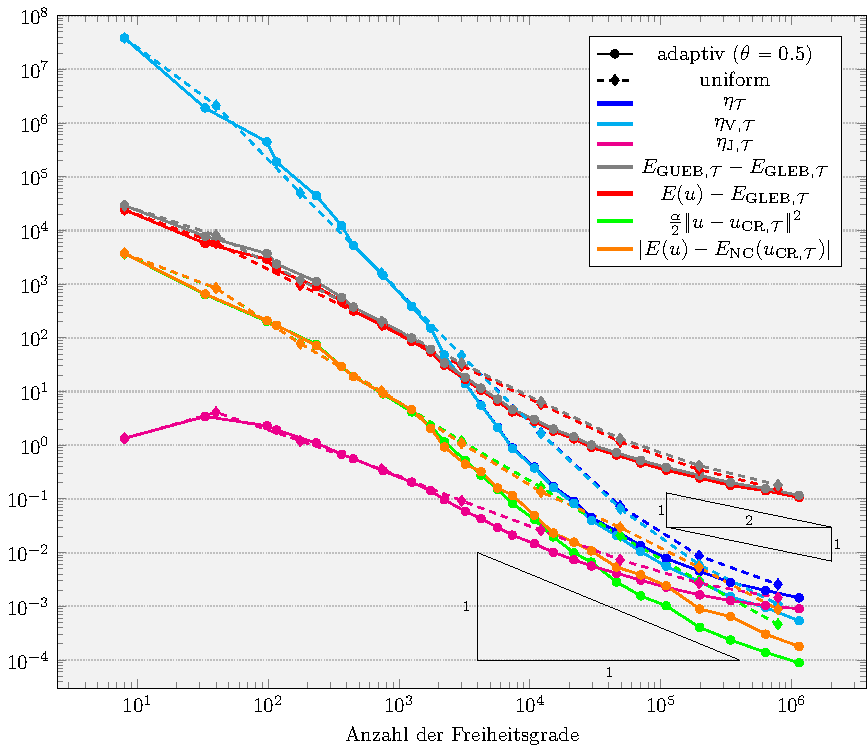
\includegraphics[width=\linewidth]
    {pictures/chapExperiments/secExactSol/f01LargeAlpha/conv.pdf}
  \caption{Ergebnisse der adaptiven und uniformen AFEM-Schleifen für das 
  Eingangssignal $f$ mit $\alpha=10^4$.}
  \label{fig:f01LargeAlphaConvergence}
\end{figure}
Wir sehen in \Cref{fig:f01LargeAlphaConvergence} höhere Raten, welche sich 
aber ab etwa $10^4$ Freiheitsgraden veringern und schließlich ab 
circa $10^5$ Freiheitsgraden die schon in \Cref{fig:f01Convergence} 
beobachteten Raten anzunehmen scheinen. 
Die einzige Rate, die sich verbessert, ist die Energiedifferenz
$|E(u)-\Enc(\ucrt)|$ die nun statt Rate $1/2$ die Rate $1$ zu erreichen
scheint.
Ansonsten gibt es nur zwei nennenswerte Unterschiede zum vorherigen Experiment.
Zum einen dominiert der Volumenanteil hier lange den Verfeinerungsindikator, 
wobei ab etwa $10^6$ Freiheitsgraden die Dominanz des Sprunganteils zu 
beginnen scheint. 
Zum anderen erreichen alle Graphen, mit Ausnahme des exakten Fehlers und
$\etaV$,  geringere Werte bei $10^6$ Freiheitsgraden als im vorherigen
Experiment.
Es bleibt festzuhalten, dass es es einen relativ großen preasymptotischen
Bereich zu geben scheint.  
Dies könnte daran liegen, dass im Experiment mit der großen Wahl $\alpha=10^4$
die Graphen anfangs sehr groß sind und die Iterationen zu Beginn der
AFEM-Schleife starke Reduzierungen der Terme schafft.
Die Ungleich \eqref{eq:expectedInequalities} ist auch hier weiterhin gültig,
diese theoretische Eigenschaft ist also auch hier praktisch zu beobachten.
Die Unterschiede zwischen adaptiven und uniformen Algorithmus scheinen hier
minimaler als im vorherigen Experiment zu sein.

Wie zu \Cref{fig:f01Convergence} erwähnt, sind die beobachten Raten besser
als die in \cite{Bar15} für das konforme Problem vorhergesaht.
Wir vermuten, dass die hohe Regularität der Lösung $u\in H^1_0\left(
(0,1)^2\right)$ ein Faktor dafür ist.
Um den Einfluss einer noch reguläreren Funktion zu untersuchen, folgt ein
Beispiel mit exakter Lösung $u_\textrm{HR} \in H^2_0\left((0,1)^2\right)$,
gegeben durch 
\begin{align*}
  u_\textrm{HR}(r)\coloneqq 
  \begin{cases}
    1, 
    & \text{falls } r\in\left[0, \frac{1}{3}\right]\!,\\
    54r^3 - 81r^2 + 36r - 4, 
    & \text{falls } r\in\left(\frac{1}{3}, \frac{2}{3}\right]\!,\\
    0, 
    & \text{falls } r\in\left(\frac{2}{3}, \infty\right)\!.
  \end{cases}
\end{align*}
Mit der Wahl
\begin{align*}
  \sgn&(\partial_r u_\textrm{HR}(r)) 
  \coloneqq 
  \begin{cases}
    -1458r^5 + 1215r^4 - 270r^3, 
    & \text{falls } r\in\left[0, \frac{1}{3}\right]\!,\\
    -1,
    & \text{falls } r\in\left(\frac{1}{3}, \frac{2}{3}\right]\!,\\
    -243r^4 + 756r^3 - 864r^2 + 432r - 81, 
    & \text{falls } r\in\left(\frac{2}{3}, \infty\right)\!,
  \end{cases}
\end{align*}
erhalten wir die rechte Seite
\begin{align*}
  f_\textrm{HR}(r)\coloneqq 
  \begin{cases}
    \alpha + 8748r^4 - 6075r^3 + 1080r^2, 
    & \text{falls } r\in\left[0, \frac{1}{3}\right]\!,\\
    \alpha\left(54r^3 - 81r^2 + 36r - 4\right) + \frac{1}{r}, 
    & \text{falls } r\in\left(\frac{1}{3}, \frac{2}{3}\right]\!,\\
    1215r^3 - 3024r^2 + 2592r - 864 + \frac{81}{r}, 
    & \text{falls } r\in\left(\frac{2}{3}, \infty\right)\!,
  \end{cases}
\end{align*}
für die gilt $f_\textrm{HR}\in H^2_0\left((0,1)^2\right)$.
Die schwachen Ableitungen ermittel wir mithilfe der partiellen Ableitungen
\begin{align*}
  \partial_r f_\textrm{HR}(r) =
  \begin{cases}
    34992r^3 - 18225r^2 + 2160r, 
    & \text{falls } r\in\left[0, \frac{1}{3}\right]\!,\\
    \alpha\left(162r^2 - 162r + 36\right) - \frac{1}{r^2}, 
    & \text{falls } r\in\left(\frac{1}{3}, \frac{2}{3}\right]\!,\\
    3645r^2 - 6048r + 2592 - 864 - \frac{81}{r^2}, 
    & \text{falls } r\in\left(\frac{2}{3}, \infty\right)\!,
  \end{cases}
\end{align*}
und
\begin{align*}
  \partial_r u_\textrm{HR}(r) &=
  \begin{cases}
    0,
    & \text{falls } r\in\left[0, \frac{1}{3}\right]\!,\\
    162r^2 - 162r + 36, 
    & \text{falls } r\in\left(\frac{1}{3}, \frac{2}{3}\right]\!,\\
    0, 
    & \text{falls } r\in\left(\frac{2}{3}, \infty\right)\!.
  \end{cases}
\end{align*}
Als exakte Energie erhalten wir
$
\DTLloaddb{db}{data/paramsReducedStandardF04.csv}
\DTLassign{db}{1}{\exactEnergy=exactEnergy} 
\DTLgdeletedb{db}
E(u)\approx\DTLround{\exactEnergy}{\exactEnergy}{\precDTL}\exactEnergy.
$
Eingangssignal und exakte Lösung sind in \Cref{fig:f04Plots} zu sehen.
\begin{figure}[p]
  \centering
  \begin{subfigure}[b]{.48\linewidth}
    \centering
    \caption{$f_\textrm{HR}$}
    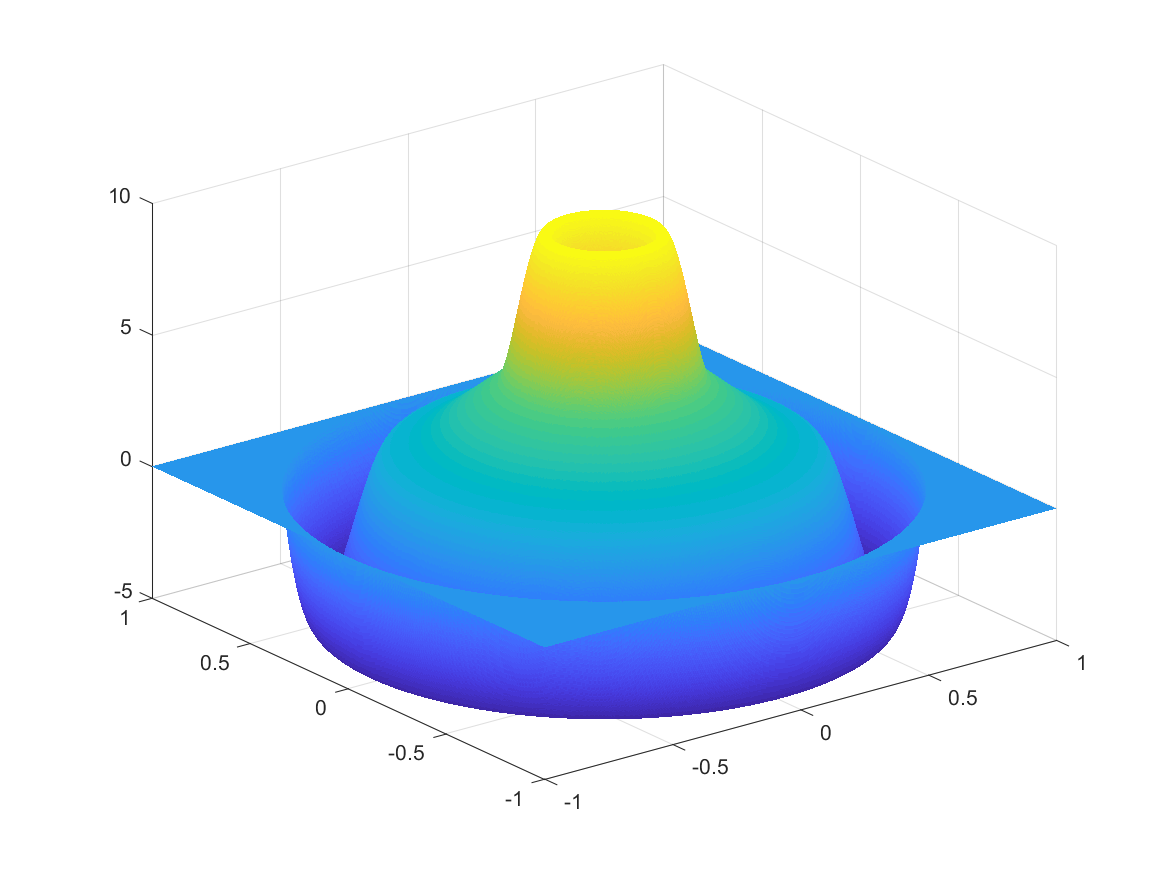
\includegraphics[trim = 40 30 30 30, clip, width=\linewidth]
      {pictures/chapExperiments/secExactSol/f04/inSi.png}
    \label{fig:f04InSi}
  \end{subfigure}
  \quad
  \begin{subfigure}[b]{.48\linewidth}
    \centering
    \caption{$f_\textrm{HR}$ entlang der x- und y-Achse}
    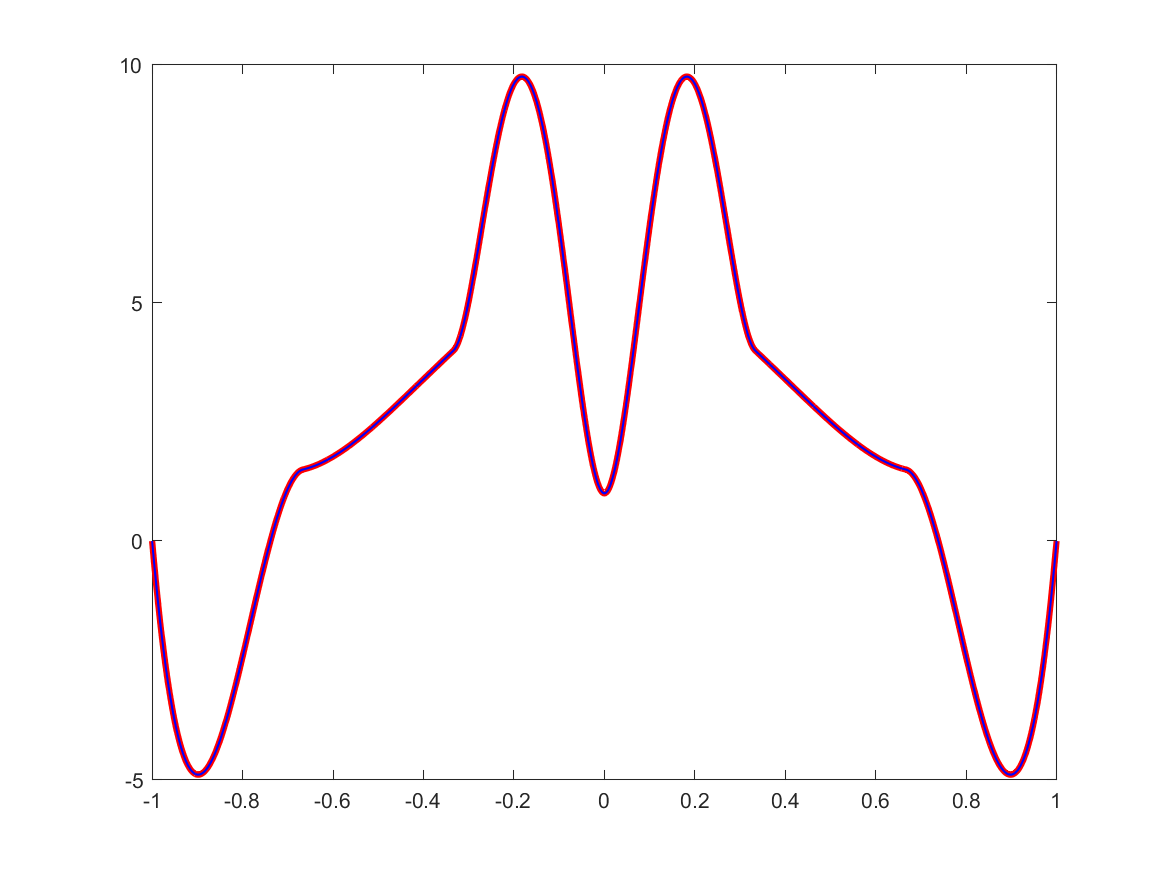
\includegraphics[trim = 50 30 50 20, clip, width=\linewidth]
      {pictures/chapExperiments/secExactSol/f04/inSiAxis.png}
    \label{fig:f04InSiAxis}
  \end{subfigure}

  \begin{subfigure}[b]{.48\linewidth}
    \centering
    \caption{$u_\textrm{HR}$}
    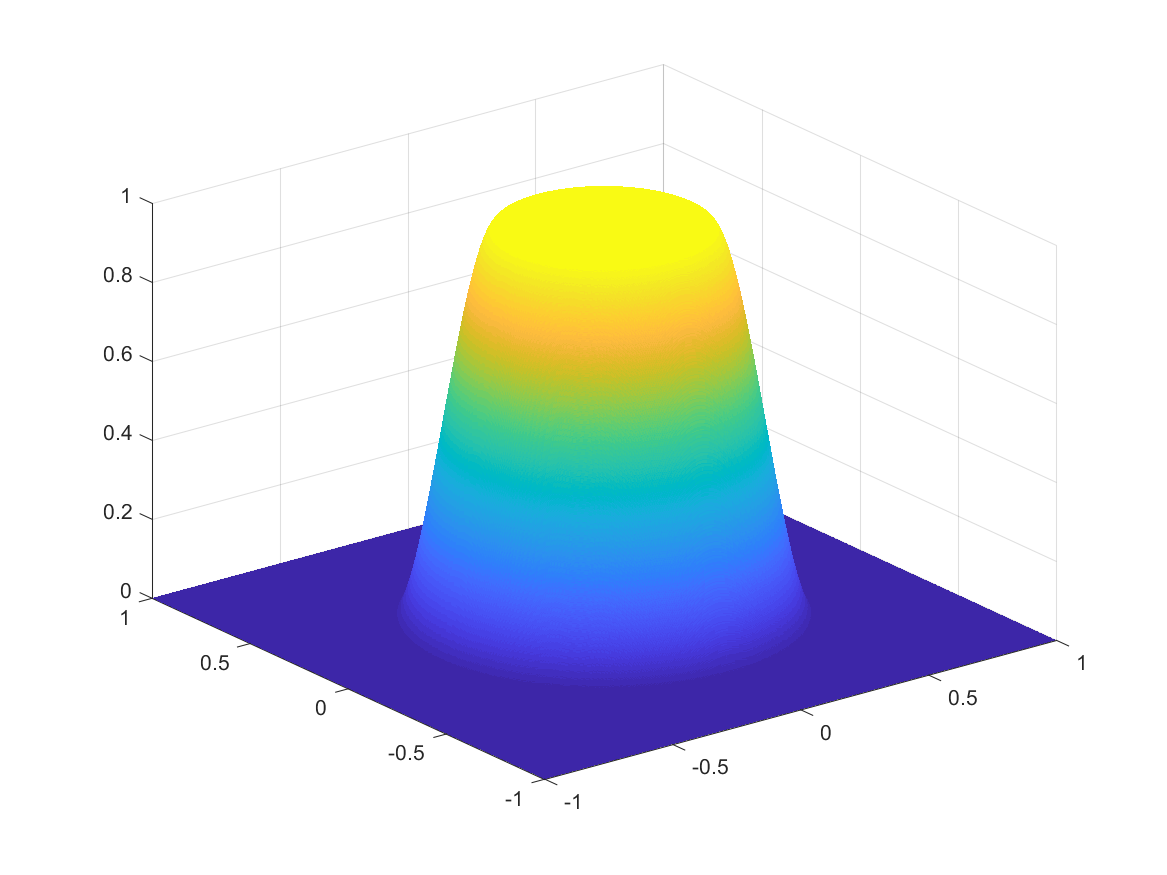
\includegraphics[trim = 40 30 30 30, clip, width=\linewidth]
      {pictures/chapExperiments/secExactSol/f04/exactSolution.png}
    \label{fig:f04ExactSol}
  \end{subfigure}
  \quad
  \begin{subfigure}[b]{.48\linewidth}
    \centering
    \caption{$u_\textrm{HR}$ entlang der x- und y-Achse}
    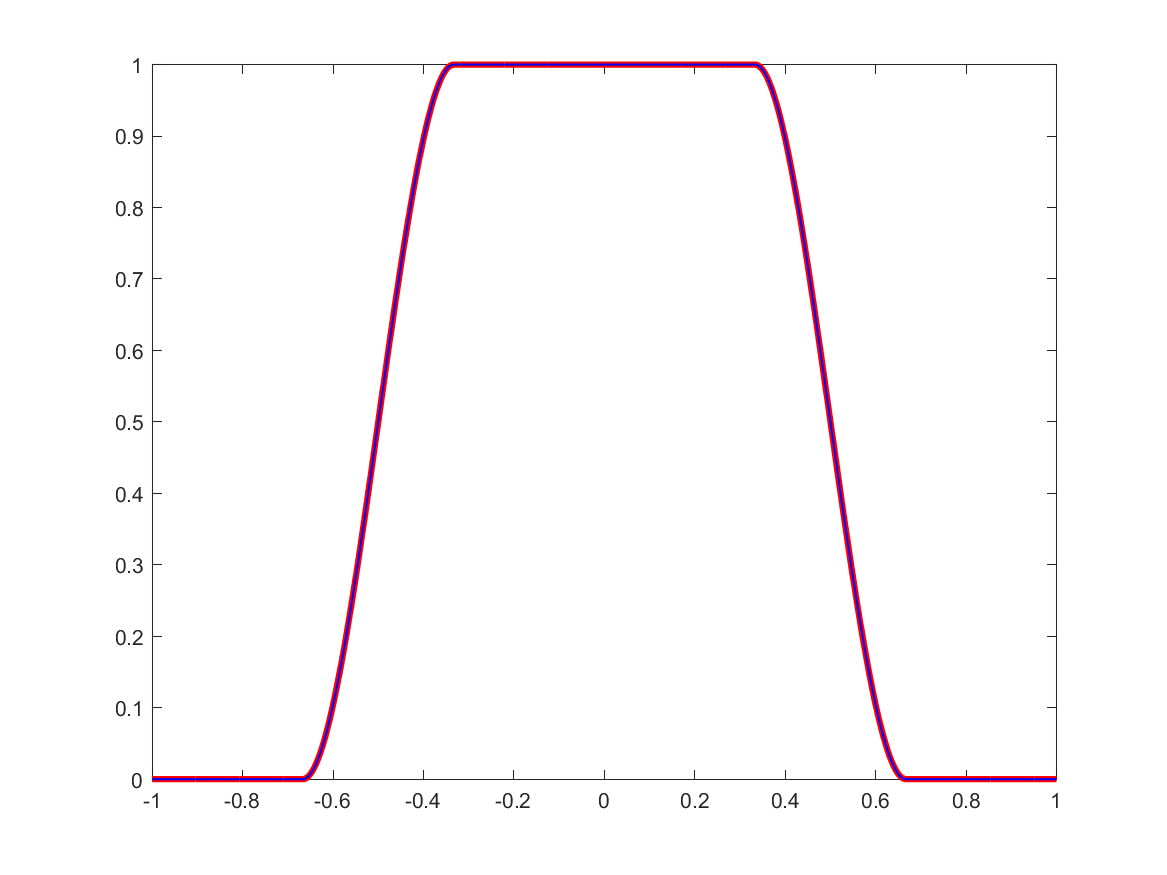
\includegraphics[trim = 50 30 50 20, clip, width=\linewidth]
      {pictures/chapExperiments/secExactSol/f04/exactSolutionAxis.png}
    \label{fig:f04ExactSolAxis}
  \end{subfigure} 
  \caption{Eingangssignal $f_\textrm{HR}$ und exakte Lösung $u_\textrm{HR}$
  sowie deren Darstellungen entlang der x-Achse (blau) und der y-Achse (rot)
  für $\alpha=1$.}
  \label{fig:f04Plots}
\end{figure}
\begin{figure}[p]
  \centering
  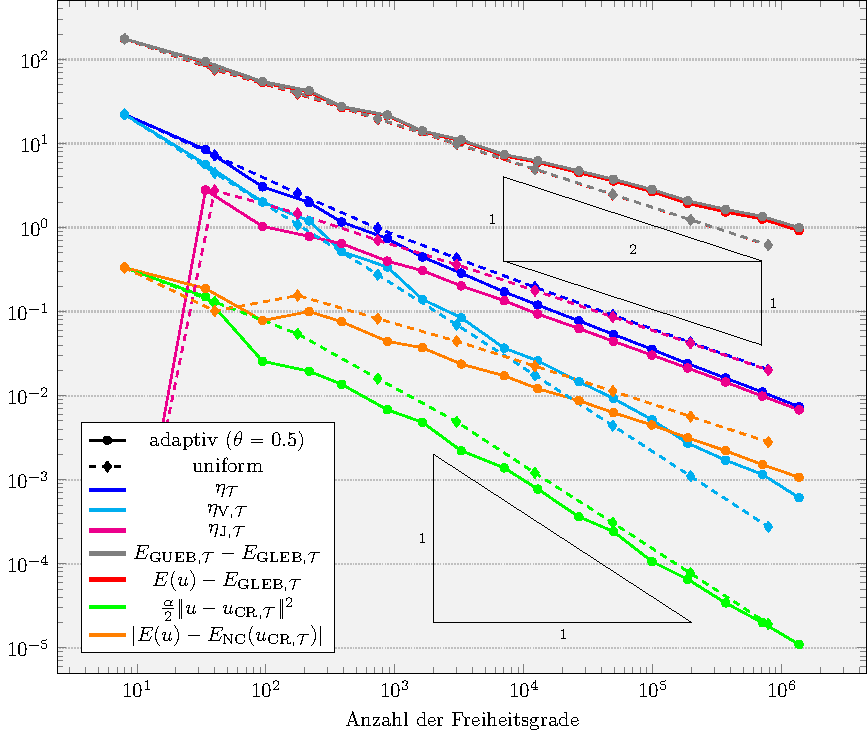
\includegraphics[width=\linewidth]
    {pictures/chapExperiments/secExactSol/f04/conv.pdf}
  \caption{Ergebnisse der adaptiven und uniformen AFEM-Schleifen für das 
  Eingangssignal $f_\textrm{HR}$.}
  \label{fig:f04Convergence}
\end{figure}
In \Cref{fig:f04Convergence} sehen wir als einzigen nennenswerten Unterschied
zu \Cref{fig:f01Convergence}, dass alle Graphen um etwa einen Faktor $10^{1/2}$
nach unten verschoben sind, also kleinere Werte erreicht werden.
Die Raten verändern sich insbesondere nicht, das heißt, eine noch stärkere
Regularitätsanname verbessert die Raten nicht weiter.

Zum Abschluss dieses Abschnitts wollen wir die drei Eingangssignale
$f_1$, $f_{10^4}$ und $f_\textup{HR}$ dieses Abschnitts in ihrem entsprechenden
Setting in der Anzahl der Iterationen vergleichen.
\begin{figure}[p]
  \centering
  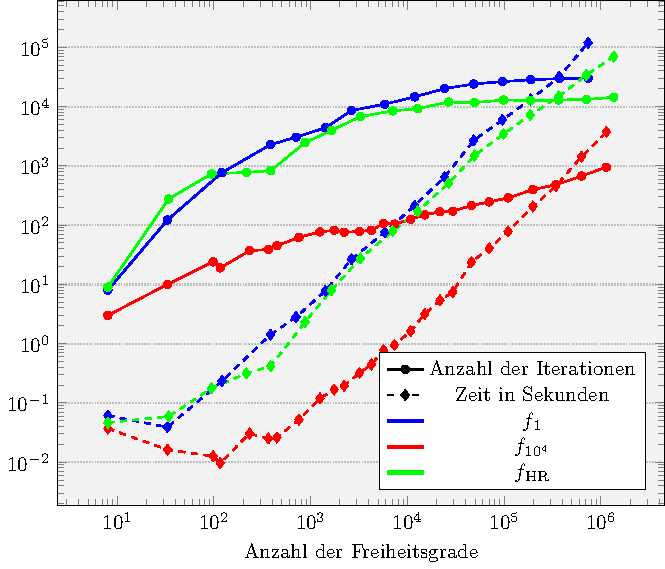
\includegraphics[width=\linewidth]
    {pictures/chapExperiments/secExactSol/nrIterComp/miscF.pdf}
  \caption{Vergleich der Iterationen fur verschiedene Eingangssignale.}
  \label{fig:inSiNrIterComparison}
\end{figure}
In \Cref{fig:inSiNrIterComparison} ist klar zu sehen, dass bis $10^6$
Freiheitsgrade das Beispiel mit Eingangssignal $f_{10^4}$, welches im Gegensatz
zu den anderen beiden Eingangssignalen den Parameter $\alpha=10^4$ nutzt,
deutlich weniger Iterationen benötigt, dafür aber mehr Level in der
AFEM-Routine durchläuft. 
Auch dies stützt unsere Hypothese aus dem
vorherigen \Cref{sec:choiceOfParameters} zum Parmeter $\tau$, denn
auch hier lässt sich feststellen, dass sich die rechte Seite der Ungleichung
\eqref{eq:nrIterationsInequality} antiproportional zur Größe von $\alpha$
verhält, was weniger Iterationsschritte zur Folge haben sollte. 
Dies ist ein zweites Indiz für die Gültigkeit der Hypothese. 
Insgesamt vermuten wir, dass eine Iteration mit möglichst wenigen
Iterationsschritten konstruiert wird, indem $\tau=1$ und $\alpha$ möglichst
groß gewählt wird.
Eine mögliche Erklärung dafür ist für den Parameter $\alpha$, dass
nach \Cref{prob:discreteProblem} für sehr große $\alpha$ die Minimierung
des Funktionals $\Vert\bullet\Vert^2$ stark gewichtet ist und die 
Minimerung der anderen Terme nicht so relevant ist.


\section{Graufarbenbilder als Eingangssignale}
\label{sec:grayscalePicturesAsInputSignal}

In diesem Abschnitt wollen wir nun auch Beispiele untersuchen, bei denen
der schwache Gradient des Eingangssignals sowie die exakte Lösung nicht bekannt
sind und prüfen, welche Aussagen wir für diese treffen können.
Unser Hauptaugenmerk liegt auf dem Eingangssignal \texttt{cameraman} aus
\Cref{fig:cameraman}. 
Insbesondere können wir an diesen Beispielen gut veranschaulichen, wie
der Verfeinerungsindikator wirkt.

\begin{figure}[p]
  \centering
  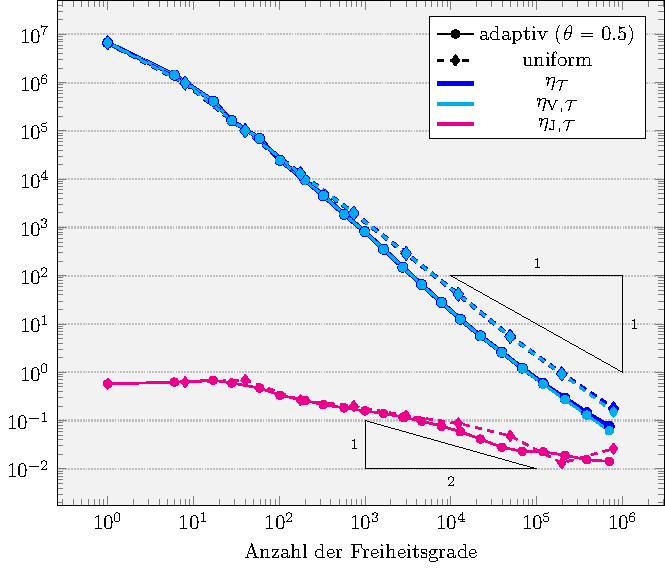
\includegraphics[width=\linewidth]
    {pictures/chapExperiments/secGrayscale/cam/conv.pdf}
  \caption{Ergebnisse der adaptiven und uniformen AFEM-Schleifen für das 
  Eingangssignal \texttt{cameraman}.}
  \label{fig:camConvergence}
\end{figure}
In \Cref{fig:camConvergence} sehen wir für den Verfeinerungsindikator und
den Volumenanteil die Rate $1$ und für den Sprunganteil die Rate $1/2$, wobei
auch hier kein Unterschied in den Raten zwischen adaptiver und uniformer
Netzverfeinerung festzustellen ist.
Die Raten von $\etaV$ und $\etaJ$ stimmen mit den Raten überein, 
die schon für das Experiment mit Eingangssignal $f_1$ in 
\Cref{fig:f01Convergence} beobachtet wurde, wobei hier im Gegensatz zu diesem
Experiment $\etaV$ dominiert und $\etaT$ entsprechend die Rate $1$ annimmt.
Ansonsten nimmt $\etaV$, und somit auch $\etaT$, zu Beginn der AFEM-Routine
deutlich höhere Werte an, vergleichbar mit dem Experiment mit in
\Cref{fig:f01LargeAlphaConvergence} mit Eingangssignal $f_{10^4}$ und,
ebenso wie hier, $\alpha=10^4$. 
Die große Wahl von $\alpha$ scheint die großen Werte für $\etaV$ also zu
beginnen, womöglich da die Eingangssignale hier deutlich höhere Werte annehmen
als die Experimente mit $\alpha=1$.
\begin{figure}[p]
  \centering
  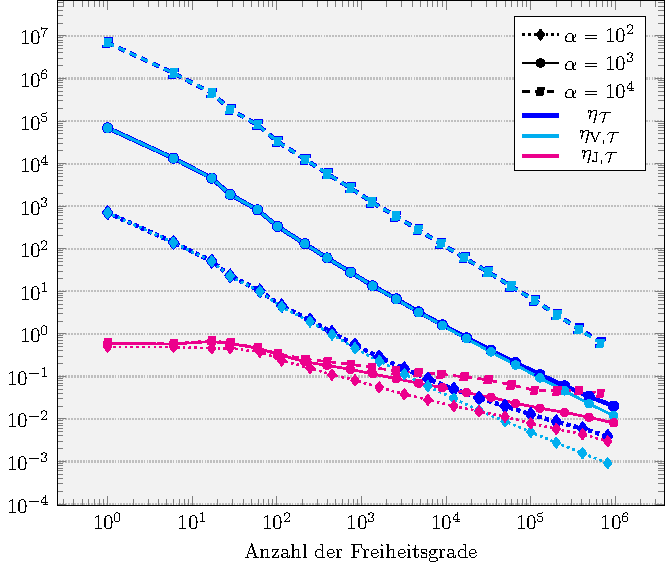
\includegraphics[width=\linewidth]
    {pictures/chapExperiments/secGrayscale/denoise/conv.pdf}
  \caption{Konvergenz im Rauschunterdrückungs Beispiel für drei verschiedene
  Werte von $\alpha$.}
  \label{fig:denoiseConvergence}
\end{figure}
Diese Vermutung wird bekräftigt in \Cref{fig:denoiseConvergence}, in der wir
zum Vergleich die Konvergenzgraphen zu \Cref{fig:exampleDenoising} angucken für
$\alpha\in\{10^2,10^3,10^4\}$.
\begin{figure}[p]
  \centering
  \begin{subfigure}[b]{.48\linewidth}
    \DTLloaddb{db}{data/currentDataReducedCamLvl17.csv}
    \DTLassign{db}{1}{\nrDof=nrDof} 
    \DTLgdeletedb{db}
    \centering
    \caption{$\text{nrDof} = \nrDof$ (Level 17)}
    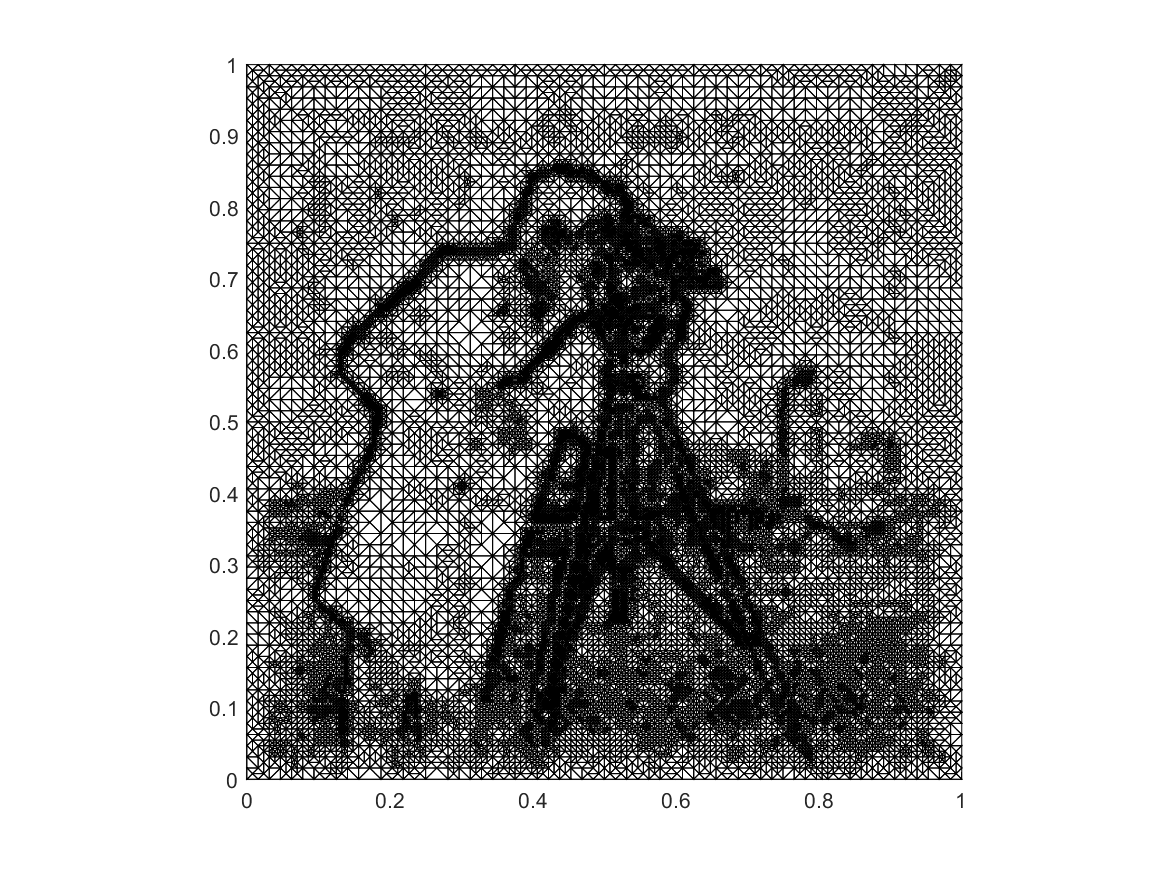
\includegraphics[trim = 100 30 80 20, clip, width=\linewidth]
      {pictures/chapExperiments/secGrayscale/cam/adaptive/lvl17/triangulation.png}
    \label{fig:camLvl17Triang}
  \end{subfigure}
  \quad
  \begin{subfigure}[b]{.48\linewidth}
    \centering
    \caption{Lösung Level 17}
    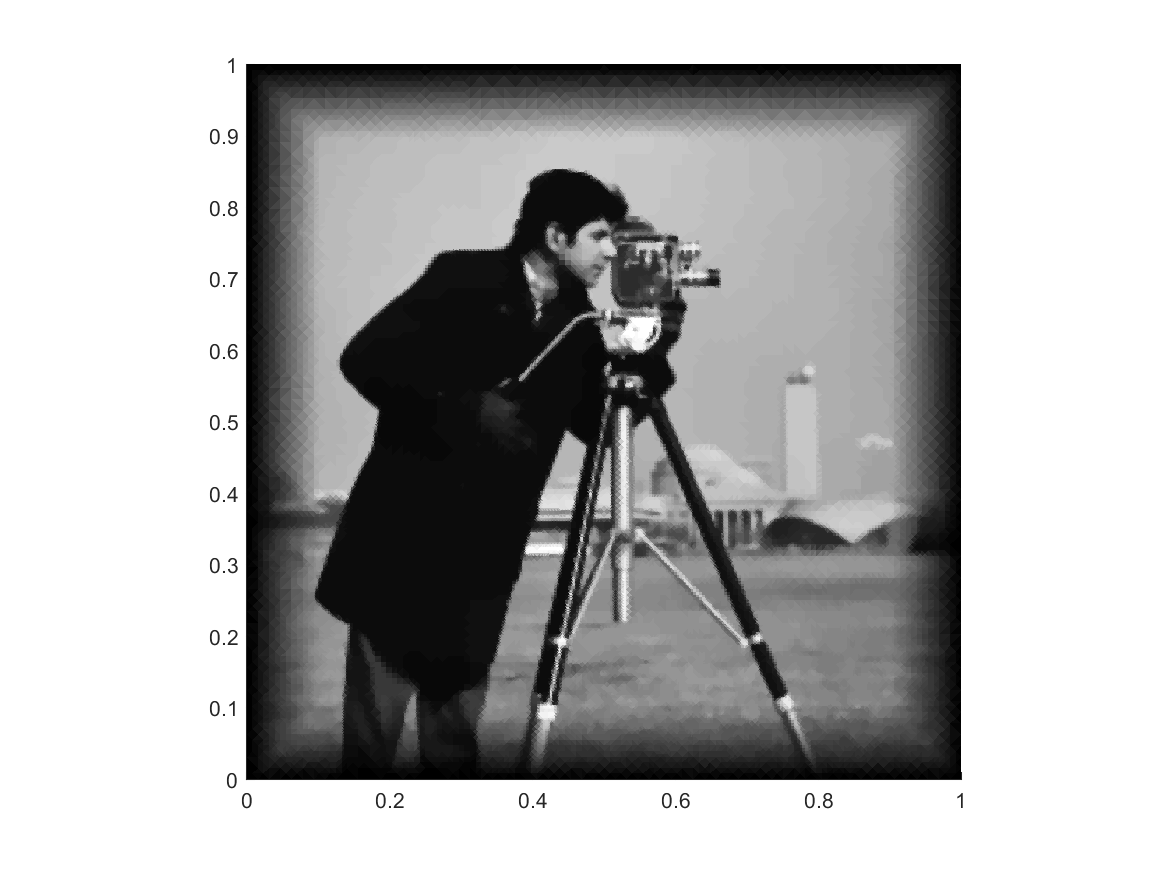
\includegraphics[trim = 100 30 80 20, clip, width=\linewidth]
      {pictures/chapExperiments/secGrayscale/cam/adaptive/lvl17/solutionGrayscale.png}
    \label{fig:camLvl17Sol}
  \end{subfigure}

  \begin{subfigure}[b]{.48\linewidth}
    \DTLloaddb{db}{data/currentDataReducedCamLvlFinal.csv}
    \DTLassign{db}{1}{\nrDof=nrDof} 
    \DTLgdeletedb{db}
    \centering
    \caption{$\text{nrDof} = \nrDof$ (Level 21)}
    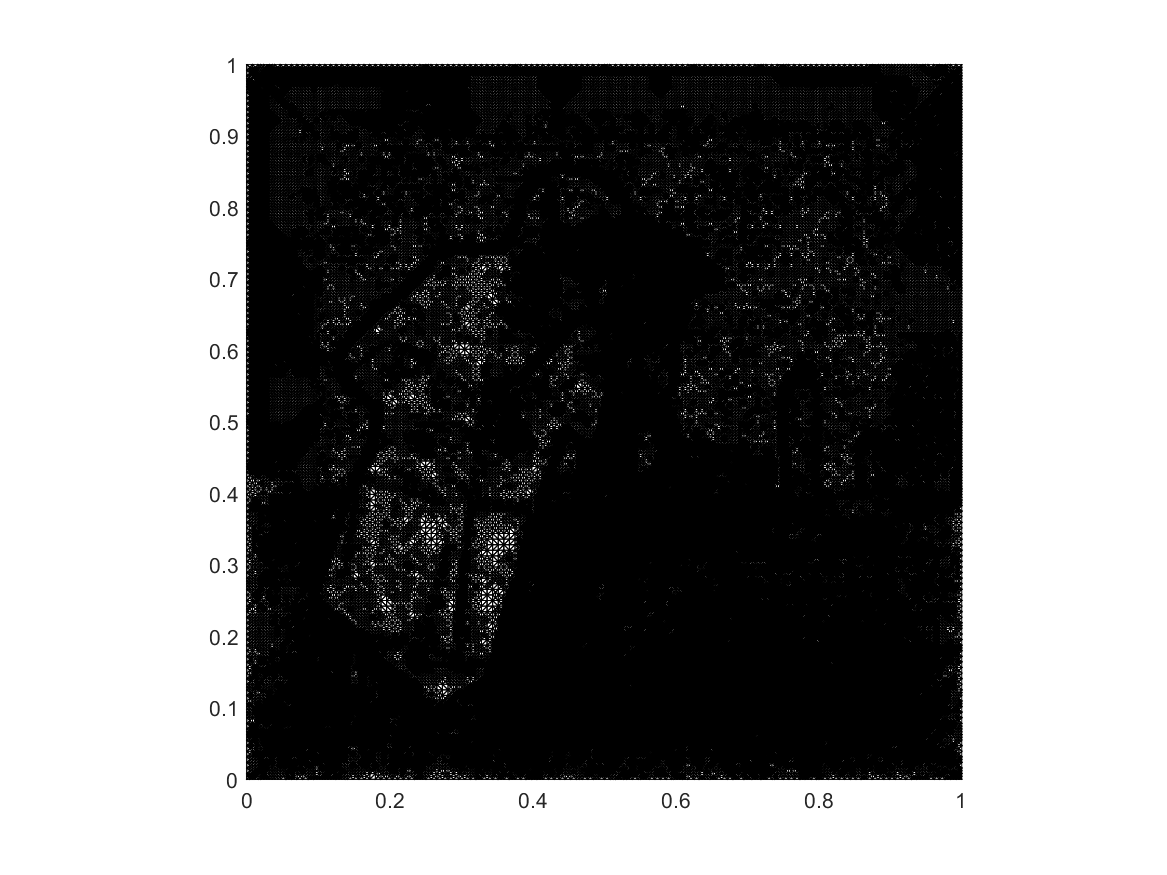
\includegraphics[trim = 100 30 80 20, clip, width=\linewidth]
      {pictures/chapExperiments/secGrayscale/cam/adaptive/lvl21/triangulation.png}
    \label{fig:camLvl21Triang}
  \end{subfigure}
  \quad
  \begin{subfigure}[b]{.48\linewidth}
    \centering
    \caption{Lösung Level 21}
    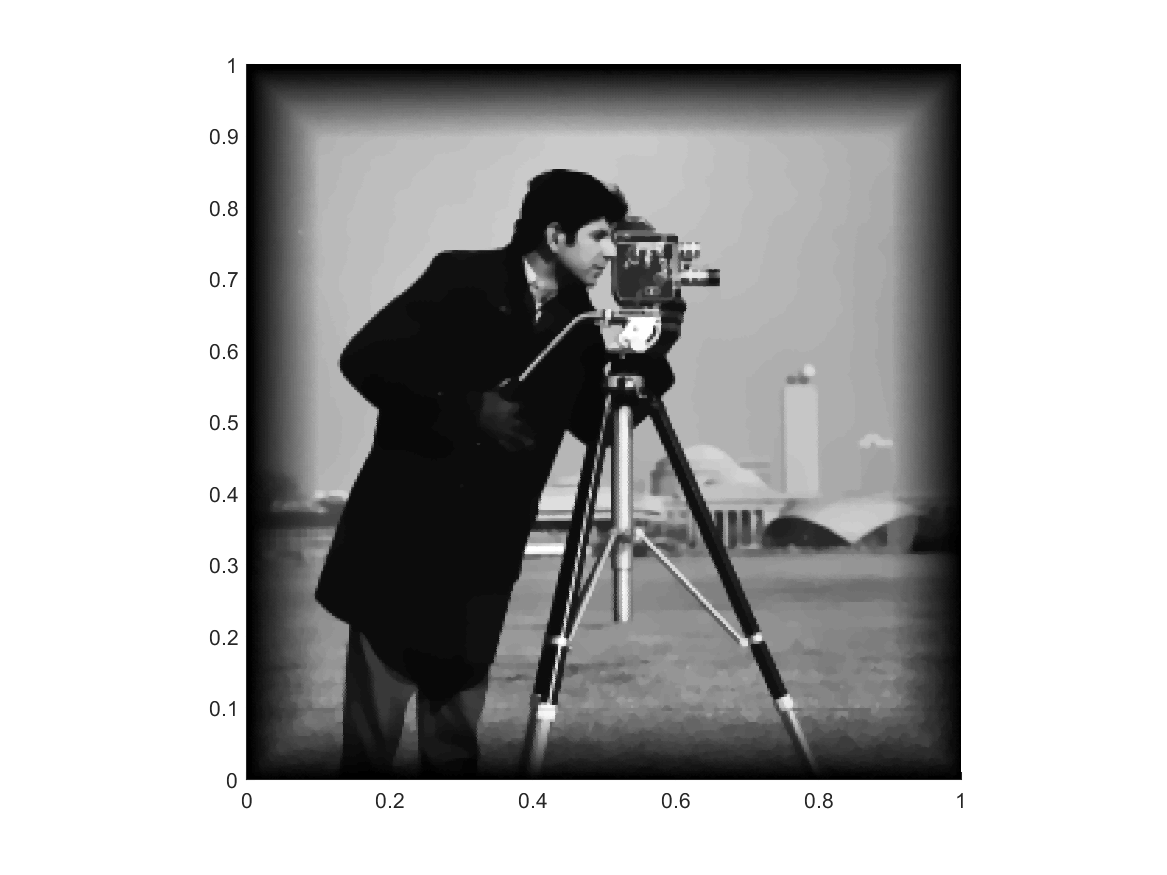
\includegraphics[trim = 100 30 80 20, clip, width=\linewidth]
      {pictures/chapExperiments/secGrayscale/cam/adaptive/lvl21/solutionGrayscale.png}
    \label{fig:camLvl21Sol}
  \end{subfigure}
  \caption{Triangulierung und Lösung für Eingangssignal \texttt{cameraman}.}
  \label{fig:camTriang}
\end{figure}
Zum Abschluss dieses Experiments noch eine Auswahl der entstandenden
Triangulierungen und den entsprechenden Lösungen des adaptiven Algorithmus für
das Eingangssignal \texttt{cameraman}, als Graufarbenplot aus der
Vogelperspektie, in \Cref{fig:camTriang}.
Wir sehen in \Cref{fig:camLvl17Triang} den Effekt des Verfeinerungsindikators
gut, der zu den Unstetigkeiten hin verfeinert, die da besonders groß sind,
wo die Farbkontraste deutlich sind. 
Weiterhin ist zu erkennen, dass der graduelle Übergang zu schwarzem Rand
den gewünschten Effekt hat, ein starke Verfeinerung am Rand, die aufgrund der 
angenommenen Nullranddaten passieren würde, zu unterdrücken.
Somit wird das Netz tatsächlich da fein, wo mehr Informationen benötigt werden,
was am Rand nicht der Fall wäre.
Auch in \Cref{fig:camLvl21Triang} kann man, trotz der hohen Anzahl
an Freiheitsgade noch erkennen, wo es im Bild kaum Farbkontraste gibt und eine
Verfeinerung deshalb nicht nötig ist.

Da wir nun gesehen haben, dass die Raten für $\etaV$ und $\etaJ$ übereinstimmen
mit den beobachteten Raten im vorherigen
\Cref{sec:experimentsWithExactSolution}, interessiert uns ob noch weitere
Raten vergleichbar sind. 
Allerdings haben wir beim Eingangssignal \texttt{cameraman} das Problem,
weder Gradienten noch die exakte Lösung zu kennen und so entsprechend keine
der anderen Graphen plotten zu können.
Deshalb betrachten wir ein weiteres Beispiel mit Unstetigkeitsmenge und 
eine kontinuierliche Approximation dieser, für die wir nach
\Cref{sec:constructionInputSignal} eine exakte Lösung kennen.
Als unstetige Funktion, die als Graufarbenbild interpretiert einem 
weißen Kreis mit Radius $1/2$ entspricht, betrachten wir die Funktion
\begin{align*}
  f_\textrm{DC}(r)\coloneqq 
  \begin{cases}
    10^4, 
    & \text{falls } r\in \left[0,\frac{1}{2}\right]\!,\\
    0, 
    & \text{falls } r\in \left(\frac{1}{2},\infty\right)\!.
  \end{cases}
\end{align*}
Betrachten wir nun die Funktion
\begin{align*}
  u_\textrm{C}(r)\coloneqq 
  \begin{cases}
    1, 
    & \text{falls } r\in \left[0,\frac{1-\beta}{2}\right]\!,\\
    -\frac{1}{\beta}r + \frac{1+\beta}{2\beta}, 
    & \text{falls } r\in \left(\frac{1-\beta}{2}, \frac{1+\beta}{2}\right]\!,\\
    0,
    & \text{falls } r\in \left(\frac{1+\beta}{2},\infty\right)\!,
  \end{cases}
\end{align*}
erhalten wir mit der Wahl
\begin{align*}
  \sgn(\partial_r u_\textrm{C}(r)) 
  &\coloneqq 
  \begin{cases}
    \frac{4}{1-\beta}r\left(\frac{1}{1-\beta}r -1\right)\!, 
    & \text{falls } r\in \left[0,\frac{1-\beta}{2}\right]\!,\\
    -1,
    & \text{falls } r\in \left(\frac{1-\beta}{2}, \frac{1+\beta}{2}\right]\!,\\
    \frac{4}{(\beta-1)^3}
    \left( 4r^3-3(\beta+3)r^2 +6(\beta+1)r-3\beta-1\right)\!, 
    & \text{falls } r\in \left(\frac{1+\beta}{2},\infty\right)\!,
  \end{cases}
\end{align*}
die rechte Seite
\begin{align*}
  f_\textrm{C}(r)\coloneqq 
  \begin{cases}
    \alpha - \frac{4}{1-\beta}\left(\frac{3}{1-\beta}r - 2\right)\!, 
    & \text{falls } r\in \left[0,\frac{1-\beta}{2}\right]\!,\\
    -\frac{\alpha}{\beta}\left( r-\frac{1+\beta}{2} \right) +\frac{1}{r}, 
    & \text{falls } r\in \left(\frac{1-\beta}{2}, \frac{1+\beta}{2}\right]\!,\\
    \frac{-4}{(\beta-1)^3}
    \left( 16r^2 -9(\beta+3)r + 12(\beta+1) - \frac{3\beta+1}{r}\right)\!, 
    & \text{falls } r\in \left(\frac{1+\beta}{2},\infty\right)\!.
  \end{cases}
\end{align*}
Die entsprechenden Ableitungen sind
\begin{align*}
  \partial_r f_\textrm{C}(r) &= 
  \begin{cases}
    -\frac{12}{(1-\beta)^2},&\text{wenn }0\leq r\leq\frac{1-\beta}{2},\\
    -\frac{\alpha}{\beta}-\frac{1}{r^2},&
    \text{wenn } \frac{1-\beta}{2}\leq r\leq \frac{1+\beta}{2},\\
    -\frac{4}{(1-\beta)^3}\left( 32r-9(\beta+3)+\frac{3\beta+1}{r^2} \right)\!,&
    \text{wenn } \frac{1+\beta}{2}\leq r\leq 1,\\
  \end{cases}
\end{align*}
und
\begin{align*}
  \partial_r u_\textrm{C}(r) &= 
  \begin{cases}
    0,&\text{wenn }0\leq r\leq\frac{1-\beta}{2},\\
    -\frac{1}{\beta},&
    \text{wenn } \frac{1-\beta}{2}\leq r\leq \frac{1+\beta}{2},\\
    0,&\text{wenn } \frac{1+\beta}{2}\leq r,
  \end{cases}
\end{align*}
womit wir die Energie
$
\DTLloaddb{db}{data/paramsReducedCircleContinuous.csv}
\DTLassign{db}{1}{\exactEnergy=exactEnergy} 
\DTLgdeletedb{db}
E(u)\approx\DTLround{\exactEnergy}{\exactEnergy}{\precDTL}\exactEnergy
$ für das Experiment mit $\alpha=10^4$ und $\beta = 10^{-3}$ erhalten.
\begin{figure}[p]
  \centering
  \begin{subfigure}[b]{.48\linewidth}
    \centering
    \caption{Insi circle stetig entlang der Achsen}
    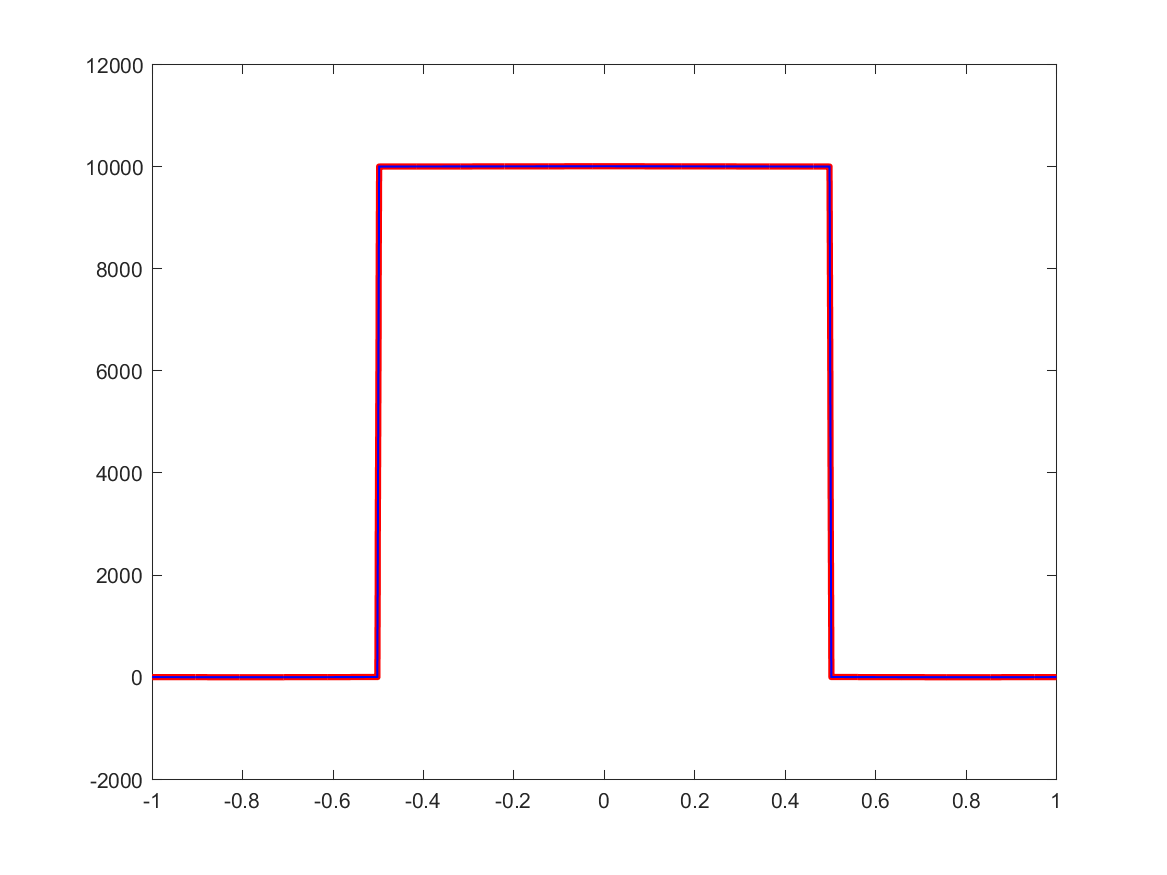
\includegraphics[trim = 40 30 50 20, clip, width=\linewidth]
      {pictures/chapExperiments/secGrayscale/circ/cont/inSiAxis.png}
    \label{fig:circContInSiAxis}
  \end{subfigure}
  \quad
  \begin{subfigure}[b]{.48\linewidth}
    \centering
    \caption{Exakte Lsg circle stetig entlang der Achsen}
    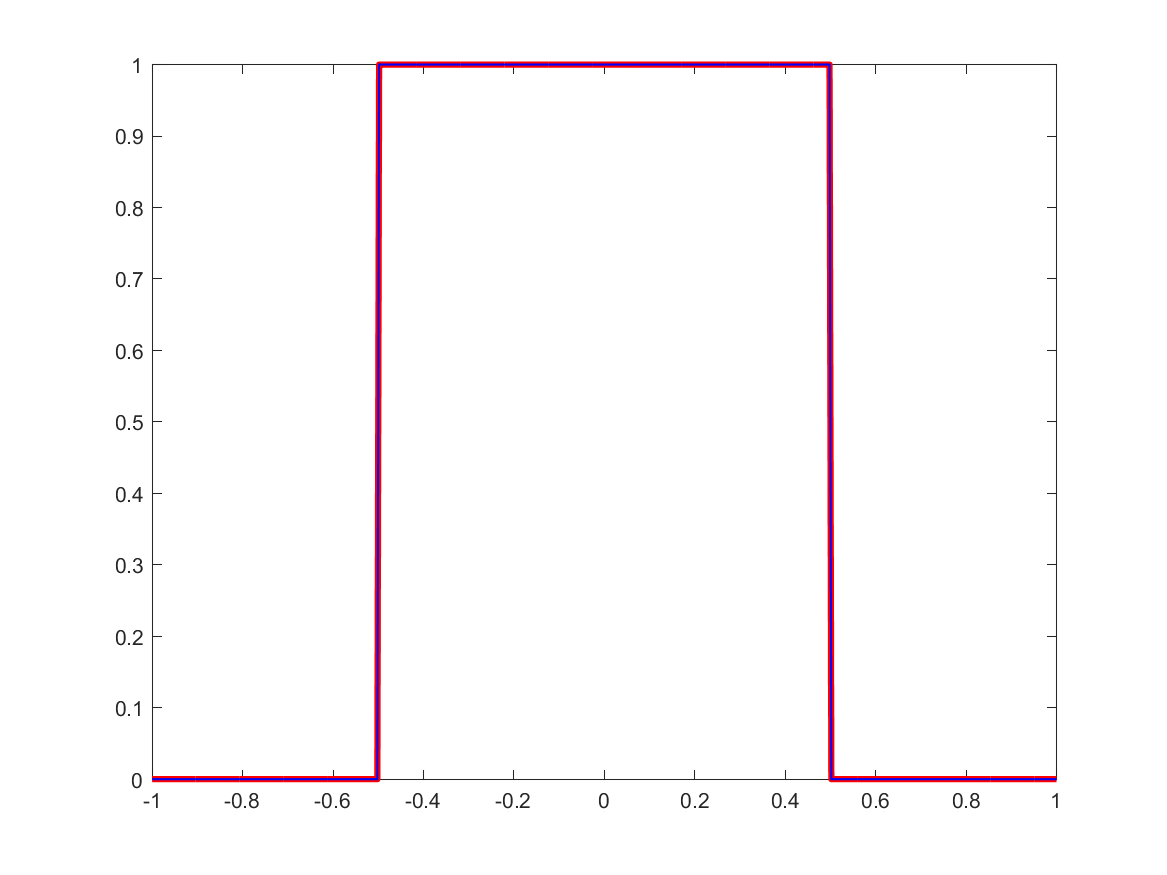
\includegraphics[trim = 40 30 50 20, clip, width=\linewidth]
      {pictures/chapExperiments/secGrayscale/circ/cont/exactSolutionAxis.png}
    \label{fig:circContExactSolAxis}
  \end{subfigure}
  \caption{InSi und exakte Lösung circle stetig entlang der Achsen.}
  \label{fig:circContPlotsAxis}
\end{figure}
Augenscheinlich ist $f_\textrm{C}$ für diese Wahl von $\alpha$ und $\beta$ eine
stetige Approximation von $f_\textrm{DC}$, wie in \Cref{fig:circContPlotsAxis}
zu sehen ist.
Außerdem sehen wir dort auch wieder für dieses große $\alpha$ das erwarte
Verhalten, dass das Eingangssignal ungefähr gleich dem Produkt aus $\alpha$ und
der exakten Lösung zu sein scheint, wie nach \Cref{chap:introduction} erwartet.
\begin{figure}[p]
  \centering
  \begin{subfigure}[b]{.48\linewidth}
    \centering
    \caption{adaptive Konvergenz vergleich stetig und unstetig}
    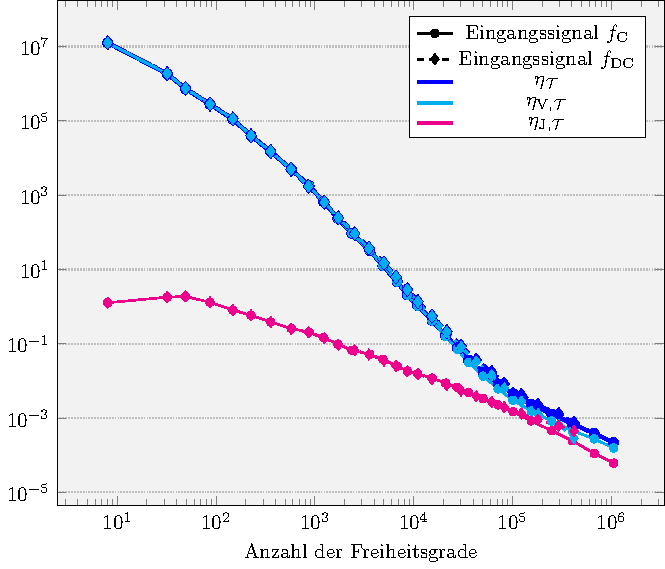
\includegraphics[width=\linewidth]
      {pictures/chapExperiments/secGrayscale/circ/convAdap.pdf}
    \label{fig:circConvAdaptive}
  \end{subfigure}
  \quad
  \begin{subfigure}[b]{.48\linewidth}
    \centering
    \caption{uniforme Konvergenz vergleich stetig und unstetig}
    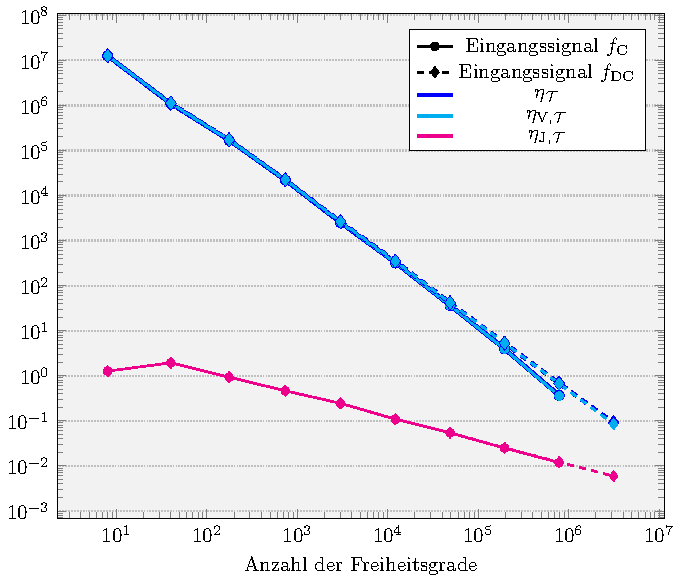
\includegraphics[width=\linewidth]
      {pictures/chapExperiments/secGrayscale/circ/convUnif.pdf}
    \label{fig:circConvUniform}
  \end{subfigure}
  \caption{adptive und uniformer Vergleich für circle stetig und unstetig}
  \label{fig:circConvComparison}
\end{figure}
Zunächst sehen wir in \Cref{fig:circConvComparison} sowohl für adaptive
als auch uniforme Netzverfeierung, dass es für die beiden Eingangssignal 
bis $10^6$ Freiheitsgrade keine deutlichen Unterschiede im Verlauf
des Verfeinerungsindikators und seiner Anteile gibt. 
\begin{figure}[p]
  \centering
  \begin{subfigure}[b]{.48\linewidth}
    \centering
    \caption{Triangulierung stetig Level 17}
    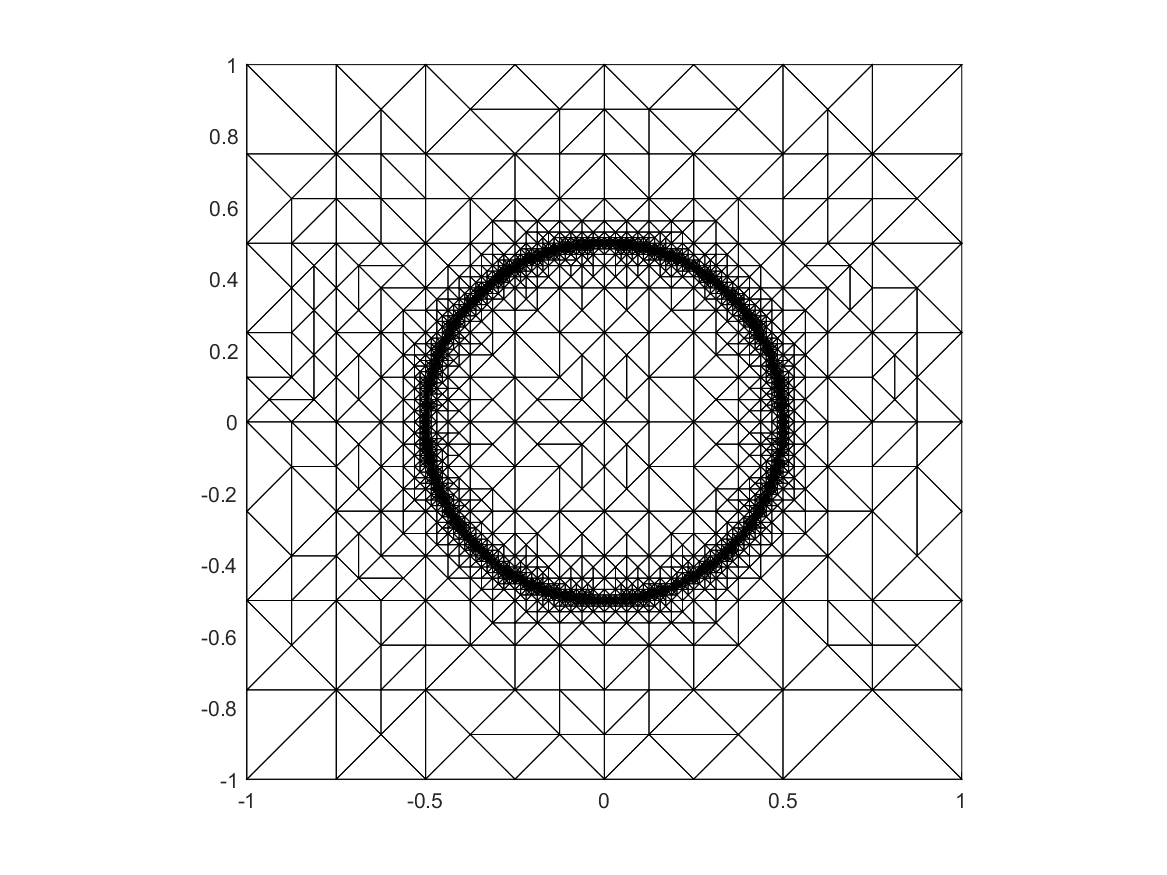
\includegraphics[trim = 100 30 80 20, clip, width=\linewidth]
      {pictures/chapExperiments/secGrayscale/circ/cont/adaptive/lvl17/triangulation.png}
    \label{fig:circContLvl17Triang}
  \end{subfigure}
  \quad
  \begin{subfigure}[b]{.48\linewidth}
    \centering
    \caption{Triangulierung unstetig Level 17}
    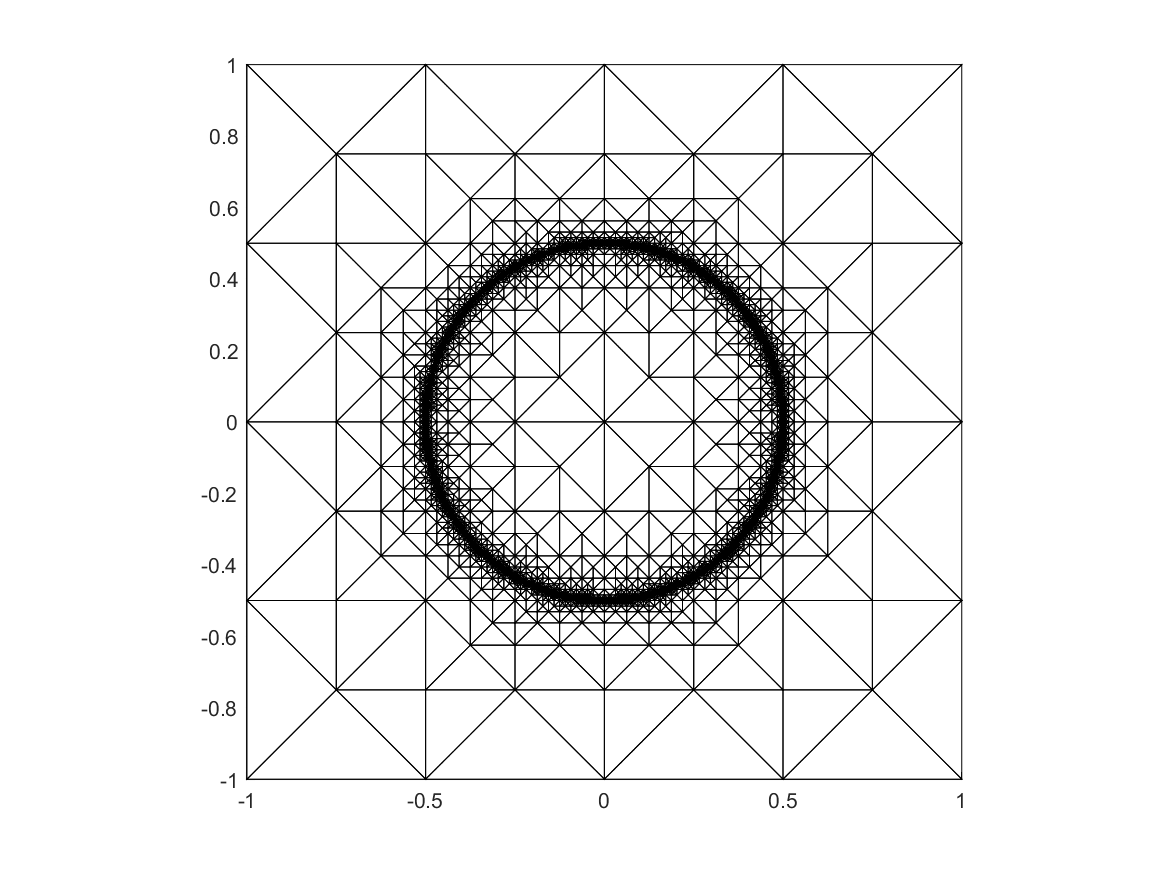
\includegraphics[trim = 100 30 80 20, clip, width=\linewidth]
      {pictures/chapExperiments/secGrayscale/circ/disc/adaptive/lvl17/triangulation.png}
    \label{fig:circDiscLvl17Triang}
  \end{subfigure}

  \begin{subfigure}[b]{.48\linewidth}
    \centering
    \caption{Triangulierung stetig Level Final}
    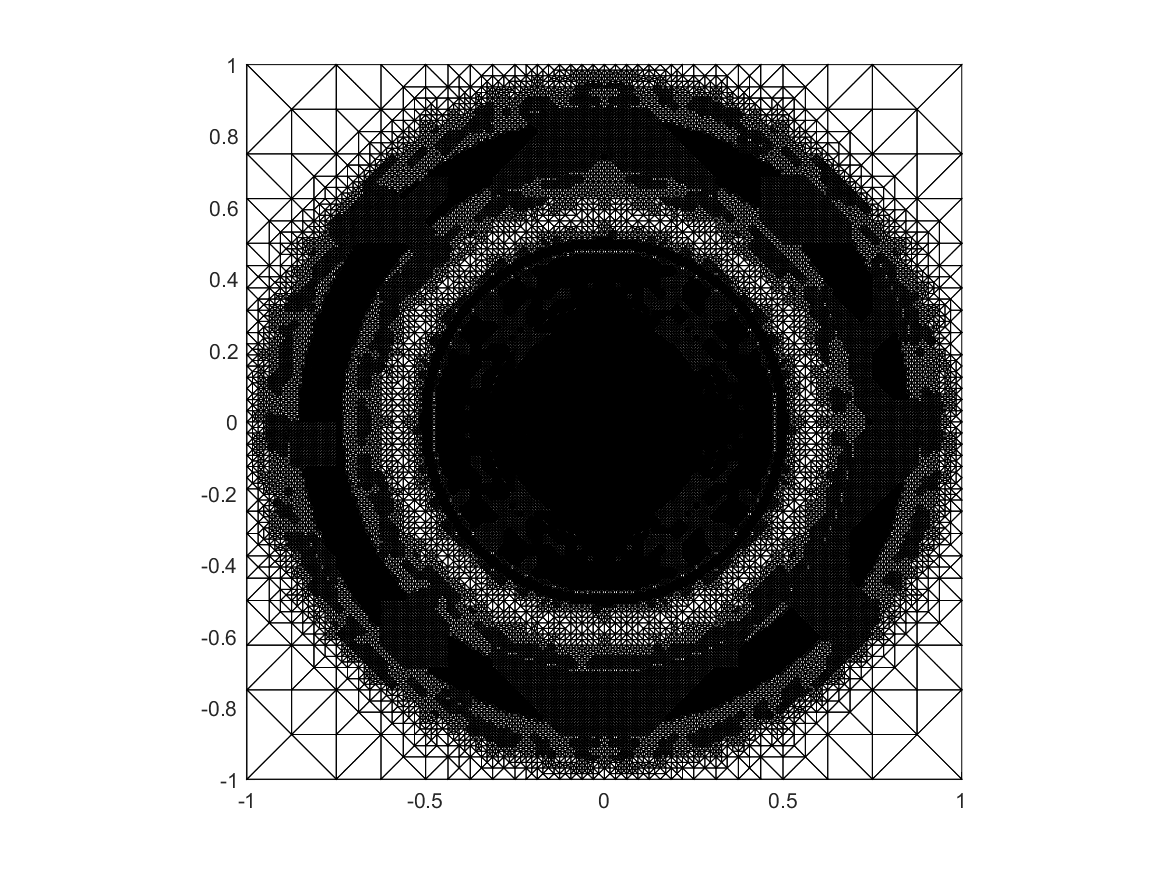
\includegraphics[trim = 100 30 80 20, clip, width=\linewidth]
      {pictures/chapExperiments/secGrayscale/circ/cont/adaptive/lvl26/triangulation.png}
    \label{fig:circContFinalTriang}
  \end{subfigure}
  \quad
  \begin{subfigure}[b]{.48\linewidth}
    \centering
    \caption{Triangulierung unstetig Level Final}
    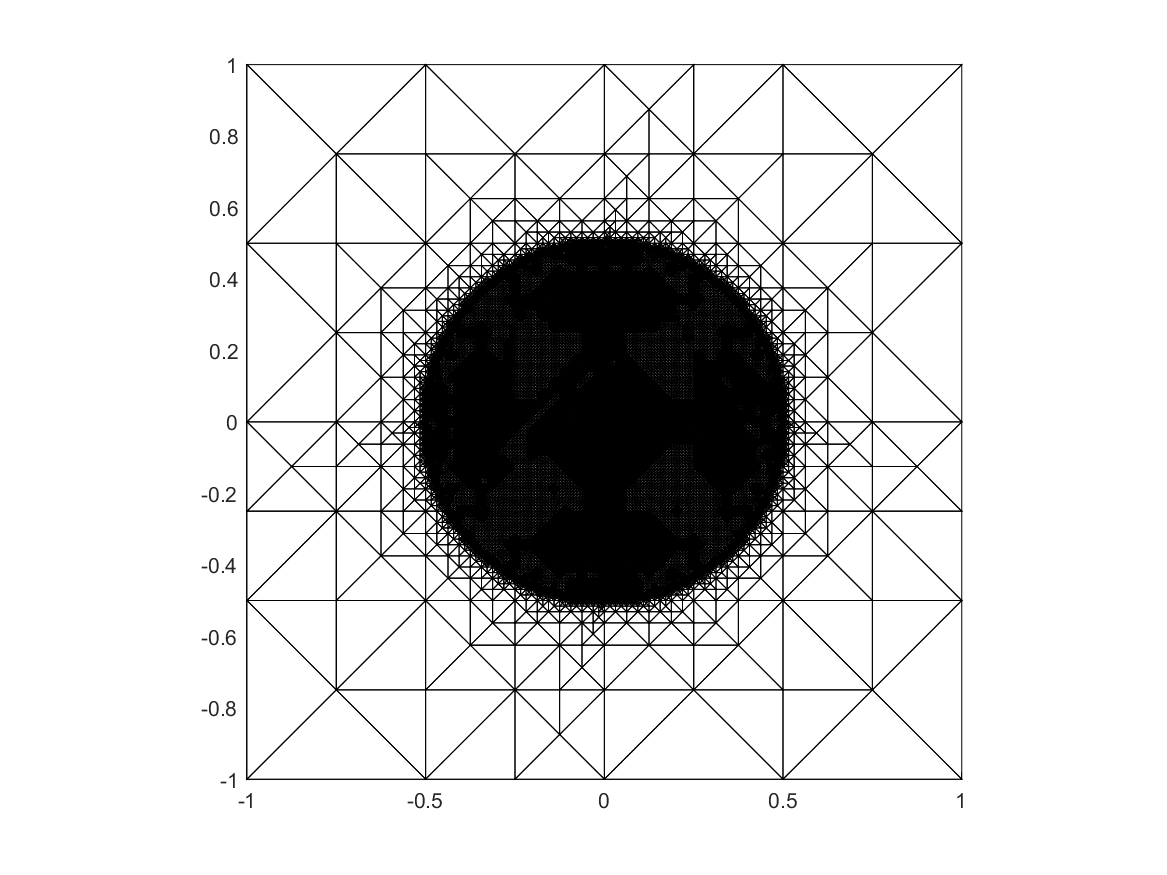
\includegraphics[trim = 100 30 80 20, clip, width=\linewidth]
      {pictures/chapExperiments/secGrayscale/circ/disc/adaptive/lvl26/triangulation.png}
    \label{fig:circDiscFinalTriang}
  \end{subfigure}
  \caption{Triangulierung für InSi circle stetig und unstetig.}
  \label{fig:circleTriang}
\end{figure}
\begin{figure}[p]
  \centering
  \begin{subfigure}[b]{.48\linewidth}
    \centering
    \caption{Lösung circ stetig}
    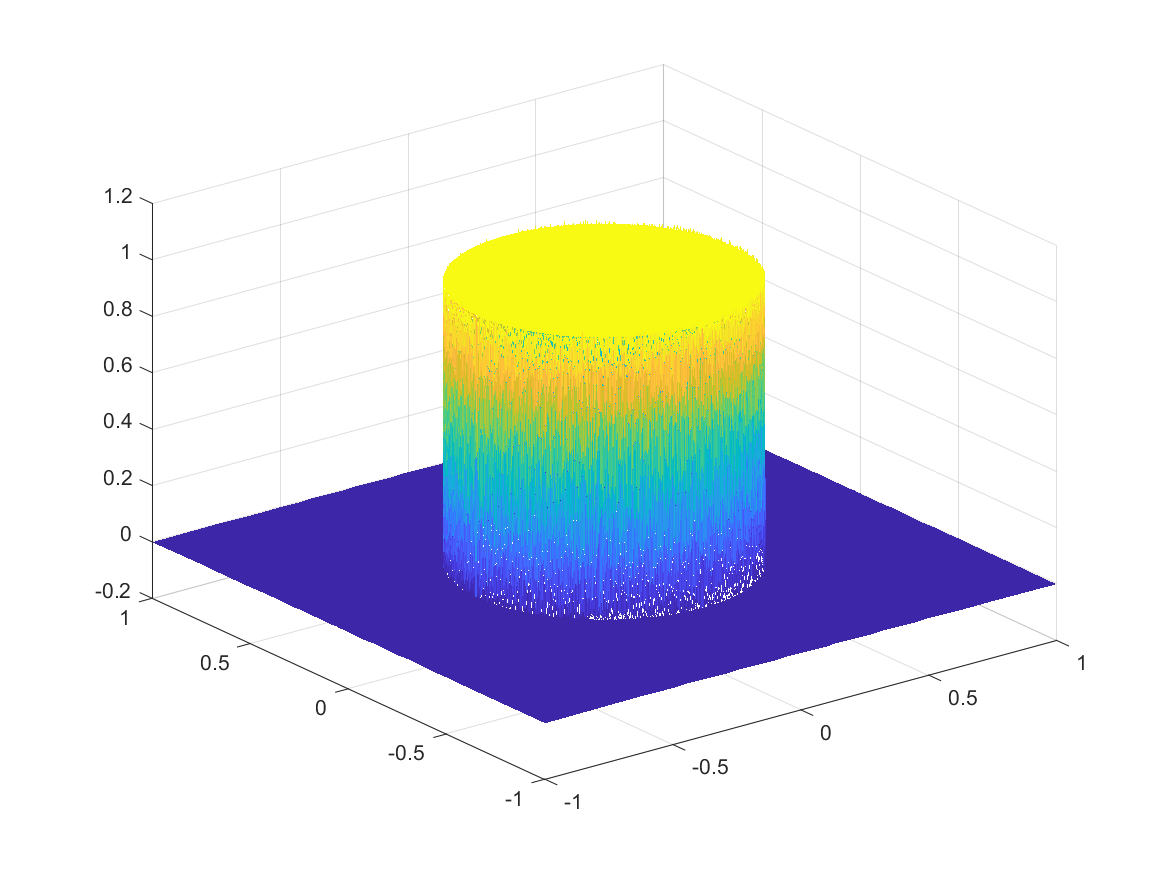
\includegraphics[trim = 40 30 30 30, clip, width=\linewidth]
      {pictures/chapExperiments/secGrayscale/circ/cont/adaptive/lvl28/solution.png}
    \label{fig:circContSol}
  \end{subfigure}
  \quad
  \begin{subfigure}[b]{.48\linewidth}
    \centering
    \caption{Lösuns stetig final entlang der Achsen}
    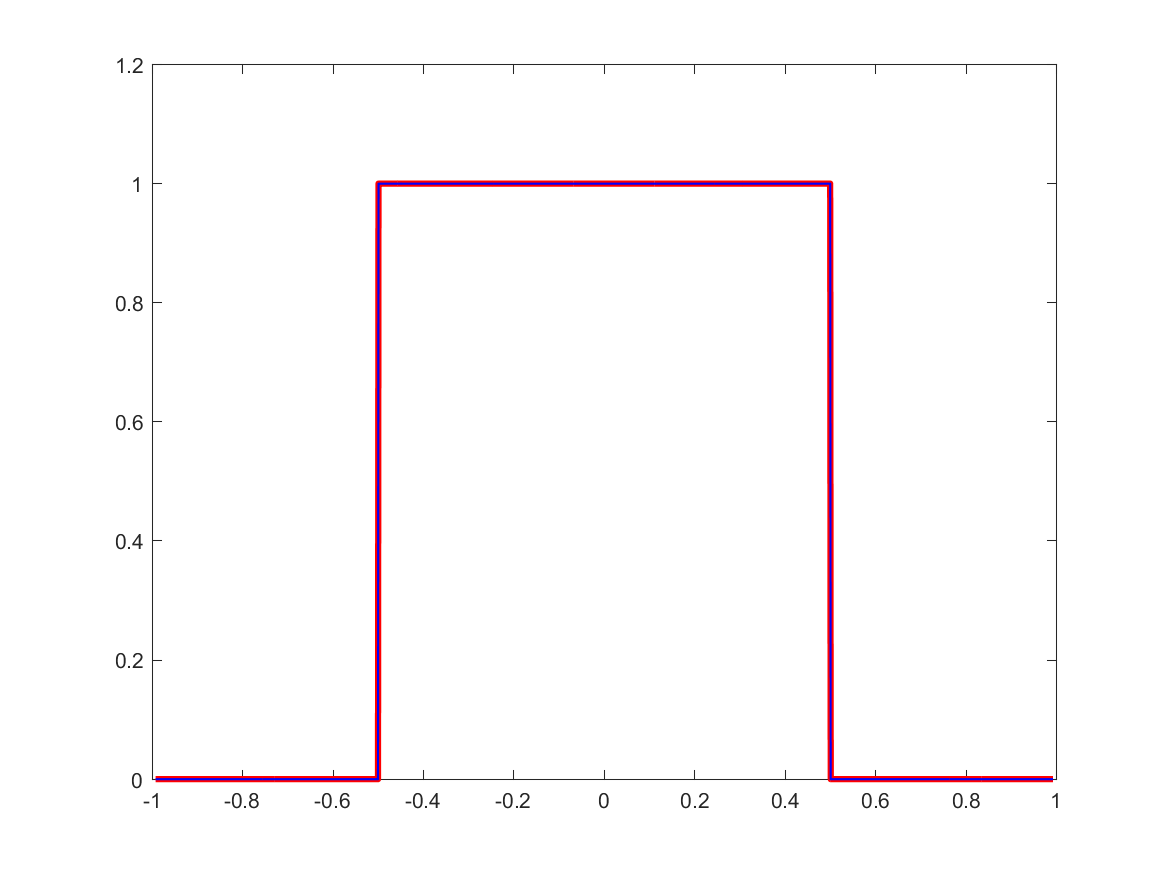
\includegraphics[trim = 50 30 50 20, clip, width=\linewidth]
      {pictures/chapExperiments/secGrayscale/circ/cont/adaptive/lvl28/solutionAxis.png}
    \label{fig:circContSolAxis}
  \end{subfigure}

  \begin{subfigure}[b]{.48\linewidth}
    \centering
    \caption{Lösung circ unstetig}
    \includegraphics[trim = 40 30 30 30, clip, width=\linewidth]
      {pictures/chapExperiments/secGrayscale/circ/disc/adaptive/lvl26/solution.png}
    \label{fig:circDiscSol}
  \end{subfigure}
  \quad
  \begin{subfigure}[b]{.48\linewidth}
    \centering
    \caption{Lösuns unstetig final entlang der Achsen}
    \includegraphics[trim = 50 30 50 20, clip, width=\linewidth]
      {pictures/chapExperiments/secGrayscale/circ/disc/adaptive/lvl26/solutionAxis.png}
    \label{fig:circDiscSolAxis}
  \end{subfigure}
  \caption{Lösung für Eingangssignal circle stetig und unstetig, wobei die
  augenscheinliche Stetigkeit der Lösung für Eingangssignal $f_\textup{DC}$
  bei $1/2$ nur durch den Plot bedingt ist.}
  \label{fig:circleSol}
\end{figure}
% TODO Freiheitsgrade ergänzen bei den Triangulierungen sobald fertig,
% außerdem auf vergleichbare Anzahl von Freiheitsgraden achten
In \Cref{fig:circleTriang} (TODO update und Freiheitsgrade ergänzen) ist
weiterhin zu sehen, dass auch der
Verfeinerungsindikator beim adaptiven Algorithmus eine vergleichbare und
erwarterte Verfeinerung zur Unstetigkeitsmenge vollzieht bei
Level 17 und sich die Verfeinerungen erst bei höheren Freiheitsgraden 
unterscheiden. 
Außerdem ähneln die in \Cref{fig:circleSol} dargestellten Lösungen der
adaptiven Algorithmen beide der exakten Lösung für das Eingangssignal
$f_\textup{C}$ aus \Cref{fig:circContExactSolAxis}.
Insgesamt scheinen die Ergebnisse beider Experiment tatsächlich vergleichbar
zu sein, weshalb wir nun das Experiment mit Eingangssignal $f_\textup{C}$
mit $\alpha=10^4$ und $\beta=10^{-3}$ weiter untersuchen möchten.
\begin{figure}[p]
  \centering
  \includegraphics[width=\linewidth]
    {pictures/chapExperiments/secGrayscale/circ/convCont.pdf}
  \caption{Ergebnisse für Eingangssignal circle stetig.}
  \label{fig:circContConvergence}
\end{figure}
In \Cref{fig:circContConvergence} ist zu sehen, dass wir hier ein Experiment
gefunden haben, bei der der adaptive Algorithmus bessere Raten als
der uniforme Algorithmus erzielt für den Fehler, die exakte Energiedifferenz
und $\etaJ$, jeweils mit Rate $1/2$ statt $1$.
Der Verfeinerungsindikator und $\etaV$ und die von $\Egleb$ abhängigen Graphen
scheinen zwar die gleichen Raten zu haben, allerdings erzielt der adaptive
Algorithmus deutlich geringere Werte.
Dies wird bei diesem Beispiel daran liegen, dass es klar nur sinnvoll sein
kann, bei der Unstetigkeit zu verfeinern, welche von der Triangulierung
natürlich nicht perfekt aufgelöst werden kann.
Diese Aussagen gelten demenstsprechend womöglich auch für $f_\textup{DC}$.
Dies zeigt, dass für Eingangssignale, bei denen
die Verfeinerung stark lokal sinnvoll ist, der adaptive Algorithmus 
ein besseres Konvergenzverhalten hat als der uniforme.
\begin{figure}[p]
  \centering
  \begin{subfigure}{.32\linewidth}
    \centering
    \caption{$f_\textup{C}$}
    \includegraphics[width=\linewidth]
      {pictures/chapExperiments/secGrayscale/circ/misc.pdf}
    \label{fig:miscCircle}
  \end{subfigure}
  \begin{subfigure}{.32\linewidth}
    \centering
    \caption{$f_1$}
    \includegraphics[width=\linewidth]
      {pictures/chapExperiments/secExactSol/f01/misc.pdf}
    \label{fig:miscF01}
  \end{subfigure}
  \begin{subfigure}{.32\linewidth}
    \centering
    \caption{\texttt{cameraman}}
    \includegraphics[width=\linewidth]
      {pictures/chapExperiments/secGrayscale/cam/misc.pdf}
    \label{fig:miscCam}
  \end{subfigure}
  \caption{Anzahl Iterationen und benötigte levelweise Zeit für drei
  Eingangssignale}
  \label{fig:miscInSi}
\end{figure}
Allerdings möchten wir an dieser Stelle auch festhalten, dass 
der adaptive Algorithmus in den hier betrachteten Expererimenten mehr Level
durchläuft und für Iterationen mit vergleichbar vielen Freiheitsgaden wie
der uniforme Algorithmus in der Regel mehr Iterationen und damit mehr
Zeit benötigt, insgesamt also mehr zeit benötigt, wie in \Cref{fig:miscInSi}
für drei Eingangssignale und insbesondere das Eingangssignal $f_\textup{C}$
zu sehen.


\section{Fazit und Ausblick}

Wir konnten in dieser Arbeit die primale-duale Iteration aus
\cite{Bar15} für eine nichtkonforme Formulierung des ROF-Modellproblems
implementieren und in numerischen Experimenten untersuchen. 
Die für die Implementierung dort garantierten Raten konnten wir deutlich 
übertreffen, auch wenn hierbei angemerkt werden muss, dass wir in den
entsprechenden Beispielen mit reguläreren Funktionen gerechnet haben
als nur Funktionen beschränkter Variation.
Ansonsten widersprachen die durch die Experimente getroffen Schlussfolgerungen
keinen in dieser Arbeit getätigten theoretischen Aussagen.
Weiterhin fanden wir experimentell Indizien, die für einige spezielle Wahlen
von Parametern für die primale-duale Iteration sprechen, insbesondere
für den Parameter $\tau$.
Das einzige Beispiel, bei dem adaptive Netzverfeinerung in der 
AFEM-Routine für einige Größen bessere Konvergenzraten erzielt als uniforme
Netzverfeinerung, war ein Beispiel mit klar definierter Unstetigkeitsmenge.
Ist Rechenzeit kein limitierender Faktor, ist davon auszugehen, dass für
solche Beispiele der adaptive Algorithmus überlegen ist.

Zum Schluss möchten wir noch einige Punkte nennen, die man als nächstes
untersuchen könnte.
\Cref{fig:parTauNoConvergence} legt nahe, über nicht konstante Wahlen für
$\tau$ nachzu\-denken, die mög\-lich\-er\-wei\-se das alternierende Verhalten in
\Cref{fig:parTauNoConvergenceEnergy} verhindern könnten.
Außerdem können die Randdaten verallgemeinert werden, um so eine größere
Menge von Beispielen betrachten zu können und insbesondere bei Bildern
als Eingangssignal keinen schwarzen Rand mehr ergänznen zu müssen. 
Das für diese Arbeit implemtierte Programm ist an einigen Stellen, zum Beispiel
beim Aufstellen der rechten Seite des Gleichungssystems in der primalen-dualen
Iteration, noch unter der Annahme optimiert, dass die Freiheitsgrade die inneren
Kanten sind.  
Dies kann aber auch aufgehoben werden.
Weiterhin kann die in \cite{Bar15} gereichte Implementierung der primalen-dualen
Iteration für die konforme Formulierung des ROF-Modellproblems angepasst werden,
um sie vergleichbar zu machen mit der Implementierung in dieser Arbeit. 
Kann man für diese noch einen Verfeinerungsindikator entwickeln, so könnte man
diese auch in einen adaptiven Algorithmus implementieren für weitere Vergleiche.
In der Theorie bleibt interessant, ob garantierte Konvergenzraten für unsere
Implementierung bewiesen werden können.

\todo[inline]{BEI allen Triangulierungsbildern die Freiheitsgrade ergänzen, mglsweise auch
bei allen Lösungsplots}
